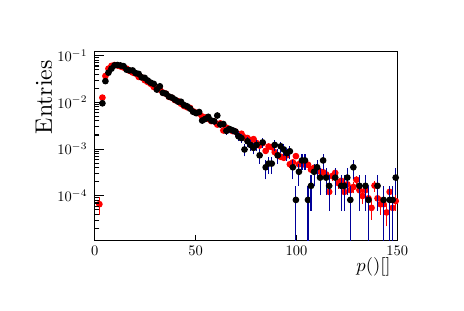
\begin{tikzpicture}
\pgfdeclareplotmark{cross} {
\pgfpathmoveto{\pgfpoint{-0.3\pgfplotmarksize}{\pgfplotmarksize}}
\pgfpathlineto{\pgfpoint{+0.3\pgfplotmarksize}{\pgfplotmarksize}}
\pgfpathlineto{\pgfpoint{+0.3\pgfplotmarksize}{0.3\pgfplotmarksize}}
\pgfpathlineto{\pgfpoint{+1\pgfplotmarksize}{0.3\pgfplotmarksize}}
\pgfpathlineto{\pgfpoint{+1\pgfplotmarksize}{-0.3\pgfplotmarksize}}
\pgfpathlineto{\pgfpoint{+0.3\pgfplotmarksize}{-0.3\pgfplotmarksize}}
\pgfpathlineto{\pgfpoint{+0.3\pgfplotmarksize}{-1.\pgfplotmarksize}}
\pgfpathlineto{\pgfpoint{-0.3\pgfplotmarksize}{-1.\pgfplotmarksize}}
\pgfpathlineto{\pgfpoint{-0.3\pgfplotmarksize}{-0.3\pgfplotmarksize}}
\pgfpathlineto{\pgfpoint{-1.\pgfplotmarksize}{-0.3\pgfplotmarksize}}
\pgfpathlineto{\pgfpoint{-1.\pgfplotmarksize}{0.3\pgfplotmarksize}}
\pgfpathlineto{\pgfpoint{-0.3\pgfplotmarksize}{0.3\pgfplotmarksize}}
\pgfpathclose
\pgfusepathqstroke
}
\pgfdeclareplotmark{cross*} {
\pgfpathmoveto{\pgfpoint{-0.3\pgfplotmarksize}{\pgfplotmarksize}}
\pgfpathlineto{\pgfpoint{+0.3\pgfplotmarksize}{\pgfplotmarksize}}
\pgfpathlineto{\pgfpoint{+0.3\pgfplotmarksize}{0.3\pgfplotmarksize}}
\pgfpathlineto{\pgfpoint{+1\pgfplotmarksize}{0.3\pgfplotmarksize}}
\pgfpathlineto{\pgfpoint{+1\pgfplotmarksize}{-0.3\pgfplotmarksize}}
\pgfpathlineto{\pgfpoint{+0.3\pgfplotmarksize}{-0.3\pgfplotmarksize}}
\pgfpathlineto{\pgfpoint{+0.3\pgfplotmarksize}{-1.\pgfplotmarksize}}
\pgfpathlineto{\pgfpoint{-0.3\pgfplotmarksize}{-1.\pgfplotmarksize}}
\pgfpathlineto{\pgfpoint{-0.3\pgfplotmarksize}{-0.3\pgfplotmarksize}}
\pgfpathlineto{\pgfpoint{-1.\pgfplotmarksize}{-0.3\pgfplotmarksize}}
\pgfpathlineto{\pgfpoint{-1.\pgfplotmarksize}{0.3\pgfplotmarksize}}
\pgfpathlineto{\pgfpoint{-0.3\pgfplotmarksize}{0.3\pgfplotmarksize}}
\pgfpathclose
\pgfusepathqfillstroke
}
\pgfdeclareplotmark{newstar} {
\pgfpathmoveto{\pgfqpoint{0pt}{\pgfplotmarksize}}
\pgfpathlineto{\pgfqpointpolar{44}{0.5\pgfplotmarksize}}
\pgfpathlineto{\pgfqpointpolar{18}{\pgfplotmarksize}}
\pgfpathlineto{\pgfqpointpolar{-20}{0.5\pgfplotmarksize}}
\pgfpathlineto{\pgfqpointpolar{-54}{\pgfplotmarksize}}
\pgfpathlineto{\pgfqpointpolar{-90}{0.5\pgfplotmarksize}}
\pgfpathlineto{\pgfqpointpolar{234}{\pgfplotmarksize}}
\pgfpathlineto{\pgfqpointpolar{198}{0.5\pgfplotmarksize}}
\pgfpathlineto{\pgfqpointpolar{162}{\pgfplotmarksize}}
\pgfpathlineto{\pgfqpointpolar{134}{0.5\pgfplotmarksize}}
\pgfpathclose
\pgfusepathqstroke
}
\pgfdeclareplotmark{newstar*} {
\pgfpathmoveto{\pgfqpoint{0pt}{\pgfplotmarksize}}
\pgfpathlineto{\pgfqpointpolar{44}{0.5\pgfplotmarksize}}
\pgfpathlineto{\pgfqpointpolar{18}{\pgfplotmarksize}}
\pgfpathlineto{\pgfqpointpolar{-20}{0.5\pgfplotmarksize}}
\pgfpathlineto{\pgfqpointpolar{-54}{\pgfplotmarksize}}
\pgfpathlineto{\pgfqpointpolar{-90}{0.5\pgfplotmarksize}}
\pgfpathlineto{\pgfqpointpolar{234}{\pgfplotmarksize}}
\pgfpathlineto{\pgfqpointpolar{198}{0.5\pgfplotmarksize}}
\pgfpathlineto{\pgfqpointpolar{162}{\pgfplotmarksize}}
\pgfpathlineto{\pgfqpointpolar{134}{0.5\pgfplotmarksize}}
\pgfpathclose
\pgfusepathqfillstroke
}
\definecolor{c}{rgb}{1,1,1};
\draw [color=c, fill=c] (5.1,3.18322) rectangle (9.9,6.17919);
\draw [color=c, fill=c] (5.58,3.48282) rectangle (9.42,5.8796);
\definecolor{c}{rgb}{0,0,0};
\draw [c] (5.58,3.48282) -- (5.58,5.8796) -- (9.42,5.8796) -- (9.42,3.48282) -- (5.58,3.48282);
\definecolor{c}{rgb}{1,0,0};
\draw [c] (5.6376,3.80931) -- (5.6376,3.9445);
\draw [c] (5.6376,3.9445) -- (5.6376,4.03271);
\draw [c] (5.6184,3.9445) -- (5.6376,3.9445);
\draw [c] (5.6376,3.9445) -- (5.6568,3.9445);
\foreach \P in {(5.6376,3.9445)}{\draw[mark options={color=c,fill=c},mark size=2.402402pt,mark=*,mark size=1pt] plot coordinates {\P};}
\draw [c] (5.676,5.29011) -- (5.676,5.29783);
\draw [c] (5.676,5.29783) -- (5.676,5.30533);
\draw [c] (5.6568,5.29783) -- (5.676,5.29783);
\draw [c] (5.676,5.29783) -- (5.6952,5.29783);
\foreach \P in {(5.676,5.29783)}{\draw[mark options={color=c,fill=c},mark size=2.402402pt,mark=*,mark size=1pt] plot coordinates {\P};}
\draw [c] (5.7144,5.56787) -- (5.7144,5.57237);
\draw [c] (5.7144,5.57237) -- (5.7144,5.5768);
\draw [c] (5.6952,5.57237) -- (5.7144,5.57237);
\draw [c] (5.7144,5.57237) -- (5.7336,5.57237);
\foreach \P in {(5.7144,5.57237)}{\draw[mark options={color=c,fill=c},mark size=2.402402pt,mark=*,mark size=1pt] plot coordinates {\P};}
\draw [c] (5.7528,5.66163) -- (5.7528,5.66539);
\draw [c] (5.7528,5.66539) -- (5.7528,5.66909);
\draw [c] (5.7336,5.66539) -- (5.7528,5.66539);
\draw [c] (5.7528,5.66539) -- (5.772,5.66539);
\foreach \P in {(5.7528,5.66539)}{\draw[mark options={color=c,fill=c},mark size=2.402402pt,mark=*,mark size=1pt] plot coordinates {\P};}
\draw [c] (5.7912,5.69744) -- (5.7912,5.70094);
\draw [c] (5.7912,5.70094) -- (5.7912,5.7044);
\draw [c] (5.772,5.70094) -- (5.7912,5.70094);
\draw [c] (5.7912,5.70094) -- (5.8104,5.70094);
\foreach \P in {(5.7912,5.70094)}{\draw[mark options={color=c,fill=c},mark size=2.402402pt,mark=*,mark size=1pt] plot coordinates {\P};}
\draw [c] (5.8296,5.70811) -- (5.8296,5.71154);
\draw [c] (5.8296,5.71154) -- (5.8296,5.71493);
\draw [c] (5.8104,5.71154) -- (5.8296,5.71154);
\draw [c] (5.8296,5.71154) -- (5.8488,5.71154);
\foreach \P in {(5.8296,5.71154)}{\draw[mark options={color=c,fill=c},mark size=2.402402pt,mark=*,mark size=1pt] plot coordinates {\P};}
\draw [c] (5.868,5.70255) -- (5.868,5.70602);
\draw [c] (5.868,5.70602) -- (5.868,5.70944);
\draw [c] (5.8488,5.70602) -- (5.868,5.70602);
\draw [c] (5.868,5.70602) -- (5.8872,5.70602);
\foreach \P in {(5.868,5.70602)}{\draw[mark options={color=c,fill=c},mark size=2.402402pt,mark=*,mark size=1pt] plot coordinates {\P};}
\draw [c] (5.9064,5.69004) -- (5.9064,5.69359);
\draw [c] (5.9064,5.69359) -- (5.9064,5.6971);
\draw [c] (5.8872,5.69359) -- (5.9064,5.69359);
\draw [c] (5.9064,5.69359) -- (5.9256,5.69359);
\foreach \P in {(5.9064,5.69359)}{\draw[mark options={color=c,fill=c},mark size=2.402402pt,mark=*,mark size=1pt] plot coordinates {\P};}
\draw [c] (5.9448,5.67684) -- (5.9448,5.68049);
\draw [c] (5.9448,5.68049) -- (5.9448,5.68409);
\draw [c] (5.9256,5.68049) -- (5.9448,5.68049);
\draw [c] (5.9448,5.68049) -- (5.964,5.68049);
\foreach \P in {(5.9448,5.68049)}{\draw[mark options={color=c,fill=c},mark size=2.402402pt,mark=*,mark size=1pt] plot coordinates {\P};}
\draw [c] (5.9832,5.66185) -- (5.9832,5.66561);
\draw [c] (5.9832,5.66561) -- (5.9832,5.66931);
\draw [c] (5.964,5.66561) -- (5.9832,5.66561);
\draw [c] (5.9832,5.66561) -- (6.0024,5.66561);
\foreach \P in {(5.9832,5.66561)}{\draw[mark options={color=c,fill=c},mark size=2.402402pt,mark=*,mark size=1pt] plot coordinates {\P};}
\draw [c] (6.0216,5.63387) -- (6.0216,5.63783);
\draw [c] (6.0216,5.63783) -- (6.0216,5.64174);
\draw [c] (6.0024,5.63783) -- (6.0216,5.63783);
\draw [c] (6.0216,5.63783) -- (6.0408,5.63783);
\foreach \P in {(6.0216,5.63783)}{\draw[mark options={color=c,fill=c},mark size=2.402402pt,mark=*,mark size=1pt] plot coordinates {\P};}
\draw [c] (6.06,5.6132) -- (6.06,5.61733);
\draw [c] (6.06,5.61733) -- (6.06,5.62139);
\draw [c] (6.0408,5.61733) -- (6.06,5.61733);
\draw [c] (6.06,5.61733) -- (6.0792,5.61733);
\foreach \P in {(6.06,5.61733)}{\draw[mark options={color=c,fill=c},mark size=2.402402pt,mark=*,mark size=1pt] plot coordinates {\P};}
\draw [c] (6.0984,5.59828) -- (6.0984,5.60253);
\draw [c] (6.0984,5.60253) -- (6.0984,5.60671);
\draw [c] (6.0792,5.60253) -- (6.0984,5.60253);
\draw [c] (6.0984,5.60253) -- (6.1176,5.60253);
\foreach \P in {(6.0984,5.60253)}{\draw[mark options={color=c,fill=c},mark size=2.402402pt,mark=*,mark size=1pt] plot coordinates {\P};}
\draw [c] (6.1368,5.55669) -- (6.1368,5.56129);
\draw [c] (6.1368,5.56129) -- (6.1368,5.56582);
\draw [c] (6.1176,5.56129) -- (6.1368,5.56129);
\draw [c] (6.1368,5.56129) -- (6.156,5.56129);
\foreach \P in {(6.1368,5.56129)}{\draw[mark options={color=c,fill=c},mark size=2.402402pt,mark=*,mark size=1pt] plot coordinates {\P};}
\draw [c] (6.1752,5.54915) -- (6.1752,5.55383);
\draw [c] (6.1752,5.55383) -- (6.1752,5.55842);
\draw [c] (6.156,5.55383) -- (6.1752,5.55383);
\draw [c] (6.1752,5.55383) -- (6.1944,5.55383);
\foreach \P in {(6.1752,5.55383)}{\draw[mark options={color=c,fill=c},mark size=2.402402pt,mark=*,mark size=1pt] plot coordinates {\P};}
\draw [c] (6.2136,5.51479) -- (6.2136,5.51979);
\draw [c] (6.2136,5.51979) -- (6.2136,5.52469);
\draw [c] (6.1944,5.51979) -- (6.2136,5.51979);
\draw [c] (6.2136,5.51979) -- (6.2328,5.51979);
\foreach \P in {(6.2136,5.51979)}{\draw[mark options={color=c,fill=c},mark size=2.402402pt,mark=*,mark size=1pt] plot coordinates {\P};}
\draw [c] (6.252,5.49162) -- (6.252,5.49685);
\draw [c] (6.252,5.49685) -- (6.252,5.50197);
\draw [c] (6.2328,5.49685) -- (6.252,5.49685);
\draw [c] (6.252,5.49685) -- (6.2712,5.49685);
\foreach \P in {(6.252,5.49685)}{\draw[mark options={color=c,fill=c},mark size=2.402402pt,mark=*,mark size=1pt] plot coordinates {\P};}
\draw [c] (6.2904,5.4671) -- (6.2904,5.47258);
\draw [c] (6.2904,5.47258) -- (6.2904,5.47795);
\draw [c] (6.2712,5.47258) -- (6.2904,5.47258);
\draw [c] (6.2904,5.47258) -- (6.3096,5.47258);
\foreach \P in {(6.2904,5.47258)}{\draw[mark options={color=c,fill=c},mark size=2.402402pt,mark=*,mark size=1pt] plot coordinates {\P};}
\draw [c] (6.3288,5.42688) -- (6.3288,5.43281);
\draw [c] (6.3288,5.43281) -- (6.3288,5.4386);
\draw [c] (6.3096,5.43281) -- (6.3288,5.43281);
\draw [c] (6.3288,5.43281) -- (6.348,5.43281);
\foreach \P in {(6.3288,5.43281)}{\draw[mark options={color=c,fill=c},mark size=2.402402pt,mark=*,mark size=1pt] plot coordinates {\P};}
\draw [c] (6.3672,5.40875) -- (6.3672,5.41489);
\draw [c] (6.3672,5.41489) -- (6.3672,5.42088);
\draw [c] (6.348,5.41489) -- (6.3672,5.41489);
\draw [c] (6.3672,5.41489) -- (6.3864,5.41489);
\foreach \P in {(6.3672,5.41489)}{\draw[mark options={color=c,fill=c},mark size=2.402402pt,mark=*,mark size=1pt] plot coordinates {\P};}
\draw [c] (6.4056,5.39404) -- (6.4056,5.40035);
\draw [c] (6.4056,5.40035) -- (6.4056,5.40651);
\draw [c] (6.3864,5.40035) -- (6.4056,5.40035);
\draw [c] (6.4056,5.40035) -- (6.4248,5.40035);
\foreach \P in {(6.4056,5.40035)}{\draw[mark options={color=c,fill=c},mark size=2.402402pt,mark=*,mark size=1pt] plot coordinates {\P};}
\draw [c] (6.444,5.35518) -- (6.444,5.36199);
\draw [c] (6.444,5.36199) -- (6.444,5.36862);
\draw [c] (6.4248,5.36199) -- (6.444,5.36199);
\draw [c] (6.444,5.36199) -- (6.4632,5.36199);
\foreach \P in {(6.444,5.36199)}{\draw[mark options={color=c,fill=c},mark size=2.402402pt,mark=*,mark size=1pt] plot coordinates {\P};}
\draw [c] (6.4824,5.34094) -- (6.4824,5.34794);
\draw [c] (6.4824,5.34794) -- (6.4824,5.35475);
\draw [c] (6.4632,5.34794) -- (6.4824,5.34794);
\draw [c] (6.4824,5.34794) -- (6.5016,5.34794);
\foreach \P in {(6.4824,5.34794)}{\draw[mark options={color=c,fill=c},mark size=2.402402pt,mark=*,mark size=1pt] plot coordinates {\P};}
\draw [c] (6.5208,5.30062) -- (6.5208,5.30819);
\draw [c] (6.5208,5.30819) -- (6.5208,5.31554);
\draw [c] (6.5016,5.30819) -- (6.5208,5.30819);
\draw [c] (6.5208,5.30819) -- (6.54,5.30819);
\foreach \P in {(6.5208,5.30819)}{\draw[mark options={color=c,fill=c},mark size=2.402402pt,mark=*,mark size=1pt] plot coordinates {\P};}
\draw [c] (6.5592,5.28735) -- (6.5592,5.29512);
\draw [c] (6.5592,5.29512) -- (6.5592,5.30266);
\draw [c] (6.54,5.29512) -- (6.5592,5.29512);
\draw [c] (6.5592,5.29512) -- (6.5784,5.29512);
\foreach \P in {(6.5592,5.29512)}{\draw[mark options={color=c,fill=c},mark size=2.402402pt,mark=*,mark size=1pt] plot coordinates {\P};}
\draw [c] (6.5976,5.25782) -- (6.5976,5.26605);
\draw [c] (6.5976,5.26605) -- (6.5976,5.27402);
\draw [c] (6.5784,5.26605) -- (6.5976,5.26605);
\draw [c] (6.5976,5.26605) -- (6.6168,5.26605);
\foreach \P in {(6.5976,5.26605)}{\draw[mark options={color=c,fill=c},mark size=2.402402pt,mark=*,mark size=1pt] plot coordinates {\P};}
\draw [c] (6.636,5.24429) -- (6.636,5.25274);
\draw [c] (6.636,5.25274) -- (6.636,5.26091);
\draw [c] (6.6168,5.25274) -- (6.636,5.25274);
\draw [c] (6.636,5.25274) -- (6.6552,5.25274);
\foreach \P in {(6.636,5.25274)}{\draw[mark options={color=c,fill=c},mark size=2.402402pt,mark=*,mark size=1pt] plot coordinates {\P};}
\draw [c] (6.6744,5.21123) -- (6.6744,5.22023);
\draw [c] (6.6744,5.22023) -- (6.6744,5.22893);
\draw [c] (6.6552,5.22023) -- (6.6744,5.22023);
\draw [c] (6.6744,5.22023) -- (6.6936,5.22023);
\foreach \P in {(6.6744,5.22023)}{\draw[mark options={color=c,fill=c},mark size=2.402402pt,mark=*,mark size=1pt] plot coordinates {\P};}
\draw [c] (6.7128,5.18283) -- (6.7128,5.19234);
\draw [c] (6.7128,5.19234) -- (6.7128,5.20152);
\draw [c] (6.6936,5.19234) -- (6.7128,5.19234);
\draw [c] (6.7128,5.19234) -- (6.732,5.19234);
\foreach \P in {(6.7128,5.19234)}{\draw[mark options={color=c,fill=c},mark size=2.402402pt,mark=*,mark size=1pt] plot coordinates {\P};}
\draw [c] (6.7512,5.16572) -- (6.7512,5.17556);
\draw [c] (6.7512,5.17556) -- (6.7512,5.18503);
\draw [c] (6.732,5.17556) -- (6.7512,5.17556);
\draw [c] (6.7512,5.17556) -- (6.7704,5.17556);
\foreach \P in {(6.7512,5.17556)}{\draw[mark options={color=c,fill=c},mark size=2.402402pt,mark=*,mark size=1pt] plot coordinates {\P};}
\draw [c] (6.7896,5.15672) -- (6.7896,5.16673);
\draw [c] (6.7896,5.16673) -- (6.7896,5.17637);
\draw [c] (6.7704,5.16673) -- (6.7896,5.16673);
\draw [c] (6.7896,5.16673) -- (6.8088,5.16673);
\foreach \P in {(6.7896,5.16673)}{\draw[mark options={color=c,fill=c},mark size=2.402402pt,mark=*,mark size=1pt] plot coordinates {\P};}
\draw [c] (6.828,5.11279) -- (6.828,5.12369);
\draw [c] (6.828,5.12369) -- (6.828,5.13415);
\draw [c] (6.8088,5.12369) -- (6.828,5.12369);
\draw [c] (6.828,5.12369) -- (6.8472,5.12369);
\foreach \P in {(6.828,5.12369)}{\draw[mark options={color=c,fill=c},mark size=2.402402pt,mark=*,mark size=1pt] plot coordinates {\P};}
\draw [c] (6.8664,5.09456) -- (6.8664,5.10585);
\draw [c] (6.8664,5.10585) -- (6.8664,5.11667);
\draw [c] (6.8472,5.10585) -- (6.8664,5.10585);
\draw [c] (6.8664,5.10585) -- (6.8856,5.10585);
\foreach \P in {(6.8664,5.10585)}{\draw[mark options={color=c,fill=c},mark size=2.402402pt,mark=*,mark size=1pt] plot coordinates {\P};}
\draw [c] (6.9048,5.08469) -- (6.9048,5.0962);
\draw [c] (6.9048,5.0962) -- (6.9048,5.10721);
\draw [c] (6.8856,5.0962) -- (6.9048,5.0962);
\draw [c] (6.9048,5.0962) -- (6.924,5.0962);
\foreach \P in {(6.9048,5.0962)}{\draw[mark options={color=c,fill=c},mark size=2.402402pt,mark=*,mark size=1pt] plot coordinates {\P};}
\draw [c] (6.9432,5.04628) -- (6.9432,5.05868);
\draw [c] (6.9432,5.05868) -- (6.9432,5.07051);
\draw [c] (6.924,5.05868) -- (6.9432,5.05868);
\draw [c] (6.9432,5.05868) -- (6.9624,5.05868);
\foreach \P in {(6.9432,5.05868)}{\draw[mark options={color=c,fill=c},mark size=2.402402pt,mark=*,mark size=1pt] plot coordinates {\P};}
\draw [c] (6.9816,5.0319) -- (6.9816,5.04465);
\draw [c] (6.9816,5.04465) -- (6.9816,5.0568);
\draw [c] (6.9624,5.04465) -- (6.9816,5.04465);
\draw [c] (6.9816,5.04465) -- (7.0008,5.04465);
\foreach \P in {(6.9816,5.04465)}{\draw[mark options={color=c,fill=c},mark size=2.402402pt,mark=*,mark size=1pt] plot coordinates {\P};}
\draw [c] (7.02,5.01472) -- (7.02,5.0279);
\draw [c] (7.02,5.0279) -- (7.02,5.04045);
\draw [c] (7.0008,5.0279) -- (7.02,5.0279);
\draw [c] (7.02,5.0279) -- (7.0392,5.0279);
\foreach \P in {(7.02,5.0279)}{\draw[mark options={color=c,fill=c},mark size=2.402402pt,mark=*,mark size=1pt] plot coordinates {\P};}
\draw [c] (7.0584,4.98626) -- (7.0584,5.00019);
\draw [c] (7.0584,5.00019) -- (7.0584,5.0134);
\draw [c] (7.0392,5.00019) -- (7.0584,5.00019);
\draw [c] (7.0584,5.00019) -- (7.0776,5.00019);
\foreach \P in {(7.0584,5.00019)}{\draw[mark options={color=c,fill=c},mark size=2.402402pt,mark=*,mark size=1pt] plot coordinates {\P};}
\draw [c] (7.0968,4.98256) -- (7.0968,4.99659);
\draw [c] (7.0968,4.99659) -- (7.0968,5.0099);
\draw [c] (7.0776,4.99659) -- (7.0968,4.99659);
\draw [c] (7.0968,4.99659) -- (7.116,4.99659);
\foreach \P in {(7.0968,4.99659)}{\draw[mark options={color=c,fill=c},mark size=2.402402pt,mark=*,mark size=1pt] plot coordinates {\P};}
\draw [c] (7.1352,4.94069) -- (7.1352,4.95591);
\draw [c] (7.1352,4.95591) -- (7.1352,4.97028);
\draw [c] (7.116,4.95591) -- (7.1352,4.95591);
\draw [c] (7.1352,4.95591) -- (7.1544,4.95591);
\foreach \P in {(7.1352,4.95591)}{\draw[mark options={color=c,fill=c},mark size=2.402402pt,mark=*,mark size=1pt] plot coordinates {\P};}
\draw [c] (7.1736,4.95595) -- (7.1736,4.97073);
\draw [c] (7.1736,4.97073) -- (7.1736,4.9847);
\draw [c] (7.1544,4.97073) -- (7.1736,4.97073);
\draw [c] (7.1736,4.97073) -- (7.1928,4.97073);
\foreach \P in {(7.1736,4.97073)}{\draw[mark options={color=c,fill=c},mark size=2.402402pt,mark=*,mark size=1pt] plot coordinates {\P};}
\draw [c] (7.212,4.86295) -- (7.212,4.88065);
\draw [c] (7.212,4.88065) -- (7.212,4.89721);
\draw [c] (7.1928,4.88065) -- (7.212,4.88065);
\draw [c] (7.212,4.88065) -- (7.2312,4.88065);
\foreach \P in {(7.212,4.88065)}{\draw[mark options={color=c,fill=c},mark size=2.402402pt,mark=*,mark size=1pt] plot coordinates {\P};}
\draw [c] (7.2504,4.90015) -- (7.2504,4.91661);
\draw [c] (7.2504,4.91661) -- (7.2504,4.93209);
\draw [c] (7.2312,4.91661) -- (7.2504,4.91661);
\draw [c] (7.2504,4.91661) -- (7.2696,4.91661);
\foreach \P in {(7.2504,4.91661)}{\draw[mark options={color=c,fill=c},mark size=2.402402pt,mark=*,mark size=1pt] plot coordinates {\P};}
\draw [c] (7.2888,4.87105) -- (7.2888,4.88847);
\draw [c] (7.2888,4.88847) -- (7.2888,4.90479);
\draw [c] (7.2696,4.88847) -- (7.2888,4.88847);
\draw [c] (7.2888,4.88847) -- (7.308,4.88847);
\foreach \P in {(7.2888,4.88847)}{\draw[mark options={color=c,fill=c},mark size=2.402402pt,mark=*,mark size=1pt] plot coordinates {\P};}
\draw [c] (7.3272,4.8558) -- (7.3272,4.87375);
\draw [c] (7.3272,4.87375) -- (7.3272,4.89052);
\draw [c] (7.308,4.87375) -- (7.3272,4.87375);
\draw [c] (7.3272,4.87375) -- (7.3464,4.87375);
\foreach \P in {(7.3272,4.87375)}{\draw[mark options={color=c,fill=c},mark size=2.402402pt,mark=*,mark size=1pt] plot coordinates {\P};}
\draw [c] (7.3656,4.84845) -- (7.3656,4.86665);
\draw [c] (7.3656,4.86665) -- (7.3656,4.88365);
\draw [c] (7.3464,4.86665) -- (7.3656,4.86665);
\draw [c] (7.3656,4.86665) -- (7.3848,4.86665);
\foreach \P in {(7.3656,4.86665)}{\draw[mark options={color=c,fill=c},mark size=2.402402pt,mark=*,mark size=1pt] plot coordinates {\P};}
\draw [c] (7.404,4.79489) -- (7.404,4.81508);
\draw [c] (7.404,4.81508) -- (7.404,4.83381);
\draw [c] (7.3848,4.81508) -- (7.404,4.81508);
\draw [c] (7.404,4.81508) -- (7.4232,4.81508);
\foreach \P in {(7.404,4.81508)}{\draw[mark options={color=c,fill=c},mark size=2.402402pt,mark=*,mark size=1pt] plot coordinates {\P};}
\draw [c] (7.4424,4.81959) -- (7.4424,4.83884);
\draw [c] (7.4424,4.83884) -- (7.4424,4.85675);
\draw [c] (7.4232,4.83884) -- (7.4424,4.83884);
\draw [c] (7.4424,4.83884) -- (7.4616,4.83884);
\foreach \P in {(7.4424,4.83884)}{\draw[mark options={color=c,fill=c},mark size=2.402402pt,mark=*,mark size=1pt] plot coordinates {\P};}
\draw [c] (7.4808,4.77098) -- (7.4808,4.79213);
\draw [c] (7.4808,4.79213) -- (7.4808,4.81167);
\draw [c] (7.4616,4.79213) -- (7.4808,4.79213);
\draw [c] (7.4808,4.79213) -- (7.5,4.79213);
\foreach \P in {(7.4808,4.79213)}{\draw[mark options={color=c,fill=c},mark size=2.402402pt,mark=*,mark size=1pt] plot coordinates {\P};}
\draw [c] (7.5192,4.7625) -- (7.5192,4.784);
\draw [c] (7.5192,4.784) -- (7.5192,4.80384);
\draw [c] (7.5,4.784) -- (7.5192,4.784);
\draw [c] (7.5192,4.784) -- (7.5384,4.784);
\foreach \P in {(7.5192,4.784)}{\draw[mark options={color=c,fill=c},mark size=2.402402pt,mark=*,mark size=1pt] plot coordinates {\P};}
\draw [c] (7.5576,4.73336) -- (7.5576,4.75612);
\draw [c] (7.5576,4.75612) -- (7.5576,4.77702);
\draw [c] (7.5384,4.75612) -- (7.5576,4.75612);
\draw [c] (7.5576,4.75612) -- (7.5768,4.75612);
\foreach \P in {(7.5576,4.75612)}{\draw[mark options={color=c,fill=c},mark size=2.402402pt,mark=*,mark size=1pt] plot coordinates {\P};}
\draw [c] (7.596,4.74833) -- (7.596,4.77043);
\draw [c] (7.596,4.77043) -- (7.596,4.79079);
\draw [c] (7.5768,4.77043) -- (7.596,4.77043);
\draw [c] (7.596,4.77043) -- (7.6152,4.77043);
\foreach \P in {(7.596,4.77043)}{\draw[mark options={color=c,fill=c},mark size=2.402402pt,mark=*,mark size=1pt] plot coordinates {\P};}
\draw [c] (7.6344,4.6962) -- (7.6344,4.72066);
\draw [c] (7.6344,4.72066) -- (7.6344,4.74299);
\draw [c] (7.6152,4.72066) -- (7.6344,4.72066);
\draw [c] (7.6344,4.72066) -- (7.6536,4.72066);
\foreach \P in {(7.6344,4.72066)}{\draw[mark options={color=c,fill=c},mark size=2.402402pt,mark=*,mark size=1pt] plot coordinates {\P};}
\draw [c] (7.6728,4.66318) -- (7.6728,4.68925);
\draw [c] (7.6728,4.68925) -- (7.6728,4.71292);
\draw [c] (7.6536,4.68925) -- (7.6728,4.68925);
\draw [c] (7.6728,4.68925) -- (7.692,4.68925);
\foreach \P in {(7.6728,4.68925)}{\draw[mark options={color=c,fill=c},mark size=2.402402pt,mark=*,mark size=1pt] plot coordinates {\P};}
\draw [c] (7.7112,4.69398) -- (7.7112,4.71853);
\draw [c] (7.7112,4.71853) -- (7.7112,4.74095);
\draw [c] (7.692,4.71853) -- (7.7112,4.71853);
\draw [c] (7.7112,4.71853) -- (7.7304,4.71853);
\foreach \P in {(7.7112,4.71853)}{\draw[mark options={color=c,fill=c},mark size=2.402402pt,mark=*,mark size=1pt] plot coordinates {\P};}
\draw [c] (7.7496,4.59145) -- (7.7496,4.62141);
\draw [c] (7.7496,4.62141) -- (7.7496,4.64824);
\draw [c] (7.7304,4.62141) -- (7.7496,4.62141);
\draw [c] (7.7496,4.62141) -- (7.7688,4.62141);
\foreach \P in {(7.7496,4.62141)}{\draw[mark options={color=c,fill=c},mark size=2.402402pt,mark=*,mark size=1pt] plot coordinates {\P};}
\draw [c] (7.788,4.65031) -- (7.788,4.67703);
\draw [c] (7.788,4.67703) -- (7.788,4.70125);
\draw [c] (7.7688,4.67703) -- (7.788,4.67703);
\draw [c] (7.788,4.67703) -- (7.8072,4.67703);
\foreach \P in {(7.788,4.67703)}{\draw[mark options={color=c,fill=c},mark size=2.402402pt,mark=*,mark size=1pt] plot coordinates {\P};}
\draw [c] (7.8264,4.64227) -- (7.8264,4.66942);
\draw [c] (7.8264,4.66942) -- (7.8264,4.69398);
\draw [c] (7.8072,4.66942) -- (7.8264,4.66942);
\draw [c] (7.8264,4.66942) -- (7.8456,4.66942);
\foreach \P in {(7.8264,4.66942)}{\draw[mark options={color=c,fill=c},mark size=2.402402pt,mark=*,mark size=1pt] plot coordinates {\P};}
\draw [c] (7.8648,4.57443) -- (7.8648,4.6054);
\draw [c] (7.8648,4.6054) -- (7.8648,4.63304);
\draw [c] (7.8456,4.6054) -- (7.8648,4.6054);
\draw [c] (7.8648,4.6054) -- (7.884,4.6054);
\foreach \P in {(7.8648,4.6054)}{\draw[mark options={color=c,fill=c},mark size=2.402402pt,mark=*,mark size=1pt] plot coordinates {\P};}
\draw [c] (7.9032,4.53265) -- (7.9032,4.56623);
\draw [c] (7.9032,4.56623) -- (7.9032,4.59593);
\draw [c] (7.884,4.56623) -- (7.9032,4.56623);
\draw [c] (7.9032,4.56623) -- (7.9224,4.56623);
\foreach \P in {(7.9032,4.56623)}{\draw[mark options={color=c,fill=c},mark size=2.402402pt,mark=*,mark size=1pt] plot coordinates {\P};}
\draw [c] (7.9416,4.51125) -- (7.9416,4.54624);
\draw [c] (7.9416,4.54624) -- (7.9416,4.57705);
\draw [c] (7.9224,4.54624) -- (7.9416,4.54624);
\draw [c] (7.9416,4.54624) -- (7.9608,4.54624);
\foreach \P in {(7.9416,4.54624)}{\draw[mark options={color=c,fill=c},mark size=2.402402pt,mark=*,mark size=1pt] plot coordinates {\P};}
\draw [c] (7.98,4.49753) -- (7.98,4.53346);
\draw [c] (7.98,4.53346) -- (7.98,4.565);
\draw [c] (7.9608,4.53346) -- (7.98,4.53346);
\draw [c] (7.98,4.53346) -- (7.9992,4.53346);
\foreach \P in {(7.98,4.53346)}{\draw[mark options={color=c,fill=c},mark size=2.402402pt,mark=*,mark size=1pt] plot coordinates {\P};}
\draw [c] (8.0184,4.53265) -- (8.0184,4.56623);
\draw [c] (8.0184,4.56623) -- (8.0184,4.59593);
\draw [c] (7.9992,4.56623) -- (8.0184,4.56623);
\draw [c] (8.0184,4.56623) -- (8.0376,4.56623);
\foreach \P in {(8.0184,4.56623)}{\draw[mark options={color=c,fill=c},mark size=2.402402pt,mark=*,mark size=1pt] plot coordinates {\P};}
\draw [c] (8.0568,4.40932) -- (8.0568,4.45195);
\draw [c] (8.0568,4.45195) -- (8.0568,4.48853);
\draw [c] (8.0376,4.45195) -- (8.0568,4.45195);
\draw [c] (8.0568,4.45195) -- (8.076,4.45195);
\foreach \P in {(8.0568,4.45195)}{\draw[mark options={color=c,fill=c},mark size=2.402402pt,mark=*,mark size=1pt] plot coordinates {\P};}
\draw [c] (8.0952,4.43425) -- (8.0952,4.47487);
\draw [c] (8.0952,4.47487) -- (8.0952,4.50996);
\draw [c] (8.076,4.47487) -- (8.0952,4.47487);
\draw [c] (8.0952,4.47487) -- (8.1144,4.47487);
\foreach \P in {(8.0952,4.47487)}{\draw[mark options={color=c,fill=c},mark size=2.402402pt,mark=*,mark size=1pt] plot coordinates {\P};}
\draw [c] (8.1336,4.52002) -- (8.1336,4.55442);
\draw [c] (8.1336,4.55442) -- (8.1336,4.58477);
\draw [c] (8.1144,4.55442) -- (8.1336,4.55442);
\draw [c] (8.1336,4.55442) -- (8.1528,4.55442);
\foreach \P in {(8.1336,4.55442)}{\draw[mark options={color=c,fill=c},mark size=2.402402pt,mark=*,mark size=1pt] plot coordinates {\P};}
\draw [c] (8.172,4.40932) -- (8.172,4.45195);
\draw [c] (8.172,4.45195) -- (8.172,4.48853);
\draw [c] (8.1528,4.45195) -- (8.172,4.45195);
\draw [c] (8.172,4.45195) -- (8.1912,4.45195);
\foreach \P in {(8.172,4.45195)}{\draw[mark options={color=c,fill=c},mark size=2.402402pt,mark=*,mark size=1pt] plot coordinates {\P};}
\draw [c] (8.2104,4.41577) -- (8.2104,4.45788);
\draw [c] (8.2104,4.45788) -- (8.2104,4.49406);
\draw [c] (8.1912,4.45788) -- (8.2104,4.45788);
\draw [c] (8.2104,4.45788) -- (8.2296,4.45788);
\foreach \P in {(8.2104,4.45788)}{\draw[mark options={color=c,fill=c},mark size=2.402402pt,mark=*,mark size=1pt] plot coordinates {\P};}
\draw [c] (8.2488,4.40271) -- (8.2488,4.44589);
\draw [c] (8.2488,4.44589) -- (8.2488,4.48287);
\draw [c] (8.2296,4.44589) -- (8.2488,4.44589);
\draw [c] (8.2488,4.44589) -- (8.268,4.44589);
\foreach \P in {(8.2488,4.44589)}{\draw[mark options={color=c,fill=c},mark size=2.402402pt,mark=*,mark size=1pt] plot coordinates {\P};}
\draw [c] (8.2872,4.40271) -- (8.2872,4.44589);
\draw [c] (8.2872,4.44589) -- (8.2872,4.48287);
\draw [c] (8.268,4.44589) -- (8.2872,4.44589);
\draw [c] (8.2872,4.44589) -- (8.3064,4.44589);
\foreach \P in {(8.2872,4.44589)}{\draw[mark options={color=c,fill=c},mark size=2.402402pt,mark=*,mark size=1pt] plot coordinates {\P};}
\draw [c] (8.3256,4.33447) -- (8.3256,4.38375);
\draw [c] (8.3256,4.38375) -- (8.3256,4.4251);
\draw [c] (8.3064,4.38375) -- (8.3256,4.38375);
\draw [c] (8.3256,4.38375) -- (8.3448,4.38375);
\foreach \P in {(8.3256,4.38375)}{\draw[mark options={color=c,fill=c},mark size=2.402402pt,mark=*,mark size=1pt] plot coordinates {\P};}
\draw [c] (8.364,4.35919) -- (8.364,4.40617);
\draw [c] (8.364,4.40617) -- (8.364,4.44589);
\draw [c] (8.3448,4.40617) -- (8.364,4.40617);
\draw [c] (8.364,4.40617) -- (8.3832,4.40617);
\foreach \P in {(8.364,4.40617)}{\draw[mark options={color=c,fill=c},mark size=2.402402pt,mark=*,mark size=1pt] plot coordinates {\P};}
\draw [c] (8.4024,4.31663) -- (8.4024,4.36764);
\draw [c] (8.4024,4.36764) -- (8.4024,4.4102);
\draw [c] (8.3832,4.36764) -- (8.4024,4.36764);
\draw [c] (8.4024,4.36764) -- (8.4216,4.36764);
\foreach \P in {(8.4024,4.36764)}{\draw[mark options={color=c,fill=c},mark size=2.402402pt,mark=*,mark size=1pt] plot coordinates {\P};}
\draw [c] (8.4408,4.30725) -- (8.4408,4.35919);
\draw [c] (8.4408,4.35919) -- (8.4408,4.4024);
\draw [c] (8.4216,4.35919) -- (8.4408,4.35919);
\draw [c] (8.4408,4.35919) -- (8.46,4.35919);
\foreach \P in {(8.4408,4.35919)}{\draw[mark options={color=c,fill=c},mark size=2.402402pt,mark=*,mark size=1pt] plot coordinates {\P};}
\draw [c] (8.4792,4.29753) -- (8.4792,4.35046);
\draw [c] (8.4792,4.35046) -- (8.4792,4.39435);
\draw [c] (8.46,4.35046) -- (8.4792,4.35046);
\draw [c] (8.4792,4.35046) -- (8.4984,4.35046);
\foreach \P in {(8.4792,4.35046)}{\draw[mark options={color=c,fill=c},mark size=2.402402pt,mark=*,mark size=1pt] plot coordinates {\P};}
\draw [c] (8.5176,4.26607) -- (8.5176,4.32232);
\draw [c] (8.5176,4.32232) -- (8.5176,4.36846);
\draw [c] (8.4984,4.32232) -- (8.5176,4.32232);
\draw [c] (8.5176,4.32232) -- (8.5368,4.32232);
\foreach \P in {(8.5176,4.32232)}{\draw[mark options={color=c,fill=c},mark size=2.402402pt,mark=*,mark size=1pt] plot coordinates {\P};}
\draw [c] (8.556,4.00822) -- (8.556,4.10068);
\draw [c] (8.556,4.10068) -- (8.556,4.16858);
\draw [c] (8.5368,4.10068) -- (8.556,4.10068);
\draw [c] (8.556,4.10068) -- (8.5752,4.10068);
\foreach \P in {(8.556,4.10068)}{\draw[mark options={color=c,fill=c},mark size=2.402402pt,mark=*,mark size=1pt] plot coordinates {\P};}
\draw [c] (8.5944,4.24287) -- (8.5944,4.3017);
\draw [c] (8.5944,4.3017) -- (8.5944,4.34956);
\draw [c] (8.5752,4.3017) -- (8.5944,4.3017);
\draw [c] (8.5944,4.3017) -- (8.6136,4.3017);
\foreach \P in {(8.5944,4.3017)}{\draw[mark options={color=c,fill=c},mark size=2.402402pt,mark=*,mark size=1pt] plot coordinates {\P};}
\draw [c] (8.6328,4.28744) -- (8.6328,4.34142);
\draw [c] (8.6328,4.34142) -- (8.6328,4.38602);
\draw [c] (8.6136,4.34142) -- (8.6328,4.34142);
\draw [c] (8.6328,4.34142) -- (8.652,4.34142);
\foreach \P in {(8.6328,4.34142)}{\draw[mark options={color=c,fill=c},mark size=2.402402pt,mark=*,mark size=1pt] plot coordinates {\P};}
\draw [c] (8.6712,4.14127) -- (8.6712,4.21284);
\draw [c] (8.6712,4.21284) -- (8.6712,4.2688);
\draw [c] (8.652,4.21284) -- (8.6712,4.21284);
\draw [c] (8.6712,4.21284) -- (8.6904,4.21284);
\foreach \P in {(8.6712,4.21284)}{\draw[mark options={color=c,fill=c},mark size=2.402402pt,mark=*,mark size=1pt] plot coordinates {\P};}
\draw [c] (8.7096,4.17435) -- (8.7096,4.2415);
\draw [c] (8.7096,4.2415) -- (8.7096,4.29472);
\draw [c] (8.6904,4.2415) -- (8.7096,4.2415);
\draw [c] (8.7096,4.2415) -- (8.7288,4.2415);
\foreach \P in {(8.7096,4.2415)}{\draw[mark options={color=c,fill=c},mark size=2.402402pt,mark=*,mark size=1pt] plot coordinates {\P};}
\draw [c] (8.748,4.00822) -- (8.748,4.10068);
\draw [c] (8.748,4.10068) -- (8.748,4.16858);
\draw [c] (8.7288,4.10068) -- (8.748,4.10068);
\draw [c] (8.748,4.10068) -- (8.7672,4.10068);
\foreach \P in {(8.748,4.10068)}{\draw[mark options={color=c,fill=c},mark size=2.402402pt,mark=*,mark size=1pt] plot coordinates {\P};}
\draw [c] (8.7864,4.1231) -- (8.7864,4.19722);
\draw [c] (8.7864,4.19722) -- (8.7864,4.25472);
\draw [c] (8.7672,4.19722) -- (8.7864,4.19722);
\draw [c] (8.7864,4.19722) -- (8.8056,4.19722);
\foreach \P in {(8.7864,4.19722)}{\draw[mark options={color=c,fill=c},mark size=2.402402pt,mark=*,mark size=1pt] plot coordinates {\P};}
\draw [c] (8.8248,4.03533) -- (8.8248,4.1231);
\draw [c] (8.8248,4.1231) -- (8.8248,4.18844);
\draw [c] (8.8056,4.1231) -- (8.8248,4.1231);
\draw [c] (8.8248,4.1231) -- (8.844,4.1231);
\foreach \P in {(8.8248,4.1231)}{\draw[mark options={color=c,fill=c},mark size=2.402402pt,mark=*,mark size=1pt] plot coordinates {\P};}
\draw [c] (8.8632,4.08269) -- (8.8632,4.16282);
\draw [c] (8.8632,4.16282) -- (8.8632,4.22385);
\draw [c] (8.844,4.16282) -- (8.8632,4.16282);
\draw [c] (8.8632,4.16282) -- (8.8824,4.16282);
\foreach \P in {(8.8632,4.16282)}{\draw[mark options={color=c,fill=c},mark size=2.402402pt,mark=*,mark size=1pt] plot coordinates {\P};}
\draw [c] (8.9016,4.1895) -- (8.9016,4.25472);
\draw [c] (8.9016,4.25472) -- (8.9016,4.30672);
\draw [c] (8.8824,4.25472) -- (8.9016,4.25472);
\draw [c] (8.9016,4.25472) -- (8.9208,4.25472);
\foreach \P in {(8.9016,4.25472)}{\draw[mark options={color=c,fill=c},mark size=2.402402pt,mark=*,mark size=1pt] plot coordinates {\P};}
\draw [c] (8.94,4.03533) -- (8.94,4.1231);
\draw [c] (8.94,4.1231) -- (8.94,4.18844);
\draw [c] (8.9208,4.1231) -- (8.94,4.1231);
\draw [c] (8.94,4.1231) -- (8.9592,4.1231);
\foreach \P in {(8.94,4.1231)}{\draw[mark options={color=c,fill=c},mark size=2.402402pt,mark=*,mark size=1pt] plot coordinates {\P};}
\draw [c] (8.9784,3.9445) -- (8.9784,4.04897);
\draw [c] (8.9784,4.04897) -- (8.9784,4.1231);
\draw [c] (8.9592,4.04897) -- (8.9784,4.04897);
\draw [c] (8.9784,4.04897) -- (8.9976,4.04897);
\foreach \P in {(8.9784,4.04897)}{\draw[mark options={color=c,fill=c},mark size=2.402402pt,mark=*,mark size=1pt] plot coordinates {\P};}
\draw [c] (9.0168,4.03533) -- (9.0168,4.1231);
\draw [c] (9.0168,4.1231) -- (9.0168,4.18844);
\draw [c] (8.9976,4.1231) -- (9.0168,4.1231);
\draw [c] (9.0168,4.1231) -- (9.036,4.1231);
\foreach \P in {(9.0168,4.1231)}{\draw[mark options={color=c,fill=c},mark size=2.402402pt,mark=*,mark size=1pt] plot coordinates {\P};}
\draw [c] (9.0552,3.90621) -- (9.0552,4.01862);
\draw [c] (9.0552,4.01862) -- (9.0552,4.09663);
\draw [c] (9.036,4.01862) -- (9.0552,4.01862);
\draw [c] (9.0552,4.01862) -- (9.0744,4.01862);
\foreach \P in {(9.0552,4.01862)}{\draw[mark options={color=c,fill=c},mark size=2.402402pt,mark=*,mark size=1pt] plot coordinates {\P};}
\draw [c] (9.0936,3.74478) -- (9.0936,3.89752);
\draw [c] (9.0936,3.89752) -- (9.0936,3.99276);
\draw [c] (9.0744,3.89752) -- (9.0936,3.89752);
\draw [c] (9.0936,3.89752) -- (9.1128,3.89752);
\foreach \P in {(9.0936,3.89752)}{\draw[mark options={color=c,fill=c},mark size=2.402402pt,mark=*,mark size=1pt] plot coordinates {\P};}
\draw [c] (9.132,4.10363) -- (9.132,4.18059);
\draw [c] (9.132,4.18059) -- (9.132,4.23977);
\draw [c] (9.1128,4.18059) -- (9.132,4.18059);
\draw [c] (9.132,4.18059) -- (9.1512,4.18059);
\foreach \P in {(9.132,4.18059)}{\draw[mark options={color=c,fill=c},mark size=2.402402pt,mark=*,mark size=1pt] plot coordinates {\P};}
\draw [c] (9.1704,3.90621) -- (9.1704,4.01862);
\draw [c] (9.1704,4.01862) -- (9.1704,4.09663);
\draw [c] (9.1512,4.01862) -- (9.1704,4.01862);
\draw [c] (9.1704,4.01862) -- (9.1896,4.01862);
\foreach \P in {(9.1704,4.01862)}{\draw[mark options={color=c,fill=c},mark size=2.402402pt,mark=*,mark size=1pt] plot coordinates {\P};}
\draw [c] (9.2088,3.80931) -- (9.2088,3.9445);
\draw [c] (9.2088,3.9445) -- (9.2088,4.03271);
\draw [c] (9.1896,3.9445) -- (9.2088,3.9445);
\draw [c] (9.2088,3.9445) -- (9.228,3.9445);
\foreach \P in {(9.2088,3.9445)}{\draw[mark options={color=c,fill=c},mark size=2.402402pt,mark=*,mark size=1pt] plot coordinates {\P};}
\draw [c] (9.2472,3.80931) -- (9.2472,3.9445);
\draw [c] (9.2472,3.9445) -- (9.2472,4.03271);
\draw [c] (9.228,3.9445) -- (9.2472,3.9445);
\draw [c] (9.2472,3.9445) -- (9.2664,3.9445);
\foreach \P in {(9.2472,3.9445)}{\draw[mark options={color=c,fill=c},mark size=2.402402pt,mark=*,mark size=1pt] plot coordinates {\P};}
\draw [c] (9.2856,3.66142) -- (9.2856,3.84002);
\draw [c] (9.2856,3.84002) -- (9.2856,3.9445);
\draw [c] (9.2664,3.84002) -- (9.2856,3.84002);
\draw [c] (9.2856,3.84002) -- (9.3048,3.84002);
\foreach \P in {(9.2856,3.84002)}{\draw[mark options={color=c,fill=c},mark size=2.402402pt,mark=*,mark size=1pt] plot coordinates {\P};}
\draw [c] (9.324,4.00822) -- (9.324,4.10068);
\draw [c] (9.324,4.10068) -- (9.324,4.16858);
\draw [c] (9.3048,4.10068) -- (9.324,4.10068);
\draw [c] (9.324,4.10068) -- (9.3432,4.10068);
\foreach \P in {(9.324,4.10068)}{\draw[mark options={color=c,fill=c},mark size=2.402402pt,mark=*,mark size=1pt] plot coordinates {\P};}
\draw [c] (9.3624,3.74478) -- (9.3624,3.89752);
\draw [c] (9.3624,3.89752) -- (9.3624,3.99276);
\draw [c] (9.3432,3.89752) -- (9.3624,3.89752);
\draw [c] (9.3624,3.89752) -- (9.3816,3.89752);
\foreach \P in {(9.3624,3.89752)}{\draw[mark options={color=c,fill=c},mark size=2.402402pt,mark=*,mark size=1pt] plot coordinates {\P};}
\draw [c] (9.4008,3.86189) -- (9.4008,3.98422);
\draw [c] (9.4008,3.98422) -- (9.4008,4.06682);
\draw [c] (9.3816,3.98422) -- (9.4008,3.98422);
\draw [c] (9.4008,3.98422) -- (9.42,3.98422);
\foreach \P in {(9.4008,3.98422)}{\draw[mark options={color=c,fill=c},mark size=2.402402pt,mark=*,mark size=1pt] plot coordinates {\P};}
\definecolor{c}{rgb}{0,0,0};
\draw [c] (5.58,3.48282) -- (9.42,3.48282);
\draw [anchor= east] (9.42,3.14727) node[scale=0.672873, rotate=0]{$p(\pion) [\mevc]$};
\draw [c] (5.58,3.55472) -- (5.58,3.48282);
\draw [c] (6.86,3.55472) -- (6.86,3.48282);
\draw [c] (8.14,3.55472) -- (8.14,3.48282);
\draw [c] (9.42,3.55472) -- (9.42,3.48282);
\draw [anchor=base] (5.58,3.29108) node[scale=0.523346, rotate=0]{0};
\draw [anchor=base] (6.86,3.29108) node[scale=0.523346, rotate=0]{50};
\draw [anchor=base] (8.14,3.29108) node[scale=0.523346, rotate=0]{100};
\draw [anchor=base] (9.42,3.29108) node[scale=0.523346, rotate=0]{150};
\draw [c] (5.58,3.48282) -- (5.58,5.8796);
\draw [anchor= east] (4.93104,5.8796) node[scale=0.859782, rotate=90]{Entries};
\draw [c] (5.6376,3.63654) -- (5.58,3.63654);
\draw [c] (5.6376,3.74101) -- (5.58,3.74101);
\draw [c] (5.6376,3.81514) -- (5.58,3.81514);
\draw [c] (5.6376,3.87264) -- (5.58,3.87264);
\draw [c] (5.6376,3.91961) -- (5.58,3.91961);
\draw [c] (5.6376,3.95933) -- (5.58,3.95933);
\draw [c] (5.6376,3.99374) -- (5.58,3.99374);
\draw [c] (5.6376,4.02409) -- (5.58,4.02409);
\draw [c] (5.6952,4.05124) -- (5.58,4.05124);
\draw [anchor= east] (5.54928,4.05124) node[scale=0.523346, rotate=0]{$10^{-4}$};
\draw [c] (5.6376,4.22984) -- (5.58,4.22984);
\draw [c] (5.6376,4.33431) -- (5.58,4.33431);
\draw [c] (5.6376,4.40844) -- (5.58,4.40844);
\draw [c] (5.6376,4.46594) -- (5.58,4.46594);
\draw [c] (5.6376,4.51291) -- (5.58,4.51291);
\draw [c] (5.6376,4.55263) -- (5.58,4.55263);
\draw [c] (5.6376,4.58704) -- (5.58,4.58704);
\draw [c] (5.6376,4.61739) -- (5.58,4.61739);
\draw [c] (5.6952,4.64454) -- (5.58,4.64454);
\draw [anchor= east] (5.54928,4.64454) node[scale=0.523346, rotate=0]{$10^{-3}$};
\draw [c] (5.6376,4.82314) -- (5.58,4.82314);
\draw [c] (5.6376,4.92761) -- (5.58,4.92761);
\draw [c] (5.6376,5.00174) -- (5.58,5.00174);
\draw [c] (5.6376,5.05924) -- (5.58,5.05924);
\draw [c] (5.6376,5.10621) -- (5.58,5.10621);
\draw [c] (5.6376,5.14593) -- (5.58,5.14593);
\draw [c] (5.6376,5.18034) -- (5.58,5.18034);
\draw [c] (5.6376,5.21069) -- (5.58,5.21069);
\draw [c] (5.6952,5.23784) -- (5.58,5.23784);
\draw [anchor= east] (5.54928,5.23784) node[scale=0.523346, rotate=0]{$10^{-2}$};
\draw [c] (5.6376,5.41644) -- (5.58,5.41644);
\draw [c] (5.6376,5.52091) -- (5.58,5.52091);
\draw [c] (5.6376,5.59504) -- (5.58,5.59504);
\draw [c] (5.6376,5.65253) -- (5.58,5.65253);
\draw [c] (5.6376,5.69951) -- (5.58,5.69951);
\draw [c] (5.6376,5.73923) -- (5.58,5.73923);
\draw [c] (5.6376,5.77364) -- (5.58,5.77364);
\draw [c] (5.6376,5.80399) -- (5.58,5.80399);
\draw [c] (5.6952,5.83114) -- (5.58,5.83114);
\draw [anchor= east] (5.54928,5.83114) node[scale=0.523346, rotate=0]{$10^{-1}$};
\definecolor{c}{rgb}{0,0,0.6};
\draw [c] (5.676,5.20088) -- (5.676,5.22587);
\draw [c] (5.676,5.22587) -- (5.676,5.24866);
\draw [c] (5.6568,5.22587) -- (5.676,5.22587);
\draw [c] (5.676,5.22587) -- (5.6952,5.22587);
\definecolor{c}{rgb}{0,0,0};
\foreach \P in {(5.676,5.22587)}{\draw[mark options={color=c,fill=c},mark size=2.402402pt,mark=*,mark size=1pt] plot coordinates {\P};}
\definecolor{c}{rgb}{0,0,0.6};
\draw [c] (5.7144,5.4933) -- (5.7144,5.50748);
\draw [c] (5.7144,5.50748) -- (5.7144,5.52091);
\draw [c] (5.6952,5.50748) -- (5.7144,5.50748);
\draw [c] (5.7144,5.50748) -- (5.7336,5.50748);
\definecolor{c}{rgb}{0,0,0};
\foreach \P in {(5.7144,5.50748)}{\draw[mark options={color=c,fill=c},mark size=2.402402pt,mark=*,mark size=1pt] plot coordinates {\P};}
\definecolor{c}{rgb}{0,0,0.6};
\draw [c] (5.7528,5.60369) -- (5.7528,5.61513);
\draw [c] (5.7528,5.61513) -- (5.7528,5.62609);
\draw [c] (5.7336,5.61513) -- (5.7528,5.61513);
\draw [c] (5.7528,5.61513) -- (5.772,5.61513);
\definecolor{c}{rgb}{0,0,0};
\foreach \P in {(5.7528,5.61513)}{\draw[mark options={color=c,fill=c},mark size=2.402402pt,mark=*,mark size=1pt] plot coordinates {\P};}
\definecolor{c}{rgb}{0,0,0.6};
\draw [c] (5.7912,5.65579) -- (5.7912,5.66613);
\draw [c] (5.7912,5.66613) -- (5.7912,5.67607);
\draw [c] (5.772,5.66613) -- (5.7912,5.66613);
\draw [c] (5.7912,5.66613) -- (5.8104,5.66613);
\definecolor{c}{rgb}{0,0,0};
\foreach \P in {(5.7912,5.66613)}{\draw[mark options={color=c,fill=c},mark size=2.402402pt,mark=*,mark size=1pt] plot coordinates {\P};}
\definecolor{c}{rgb}{0,0,0.6};
\draw [c] (5.8296,5.69745) -- (5.8296,5.70699);
\draw [c] (5.8296,5.70699) -- (5.8296,5.71618);
\draw [c] (5.8104,5.70699) -- (5.8296,5.70699);
\draw [c] (5.8296,5.70699) -- (5.8488,5.70699);
\definecolor{c}{rgb}{0,0,0};
\foreach \P in {(5.8296,5.70699)}{\draw[mark options={color=c,fill=c},mark size=2.402402pt,mark=*,mark size=1pt] plot coordinates {\P};}
\definecolor{c}{rgb}{0,0,0.6};
\draw [c] (5.868,5.70226) -- (5.868,5.71171);
\draw [c] (5.868,5.71171) -- (5.868,5.72082);
\draw [c] (5.8488,5.71171) -- (5.868,5.71171);
\draw [c] (5.868,5.71171) -- (5.8872,5.71171);
\definecolor{c}{rgb}{0,0,0};
\foreach \P in {(5.868,5.71171)}{\draw[mark options={color=c,fill=c},mark size=2.402402pt,mark=*,mark size=1pt] plot coordinates {\P};}
\definecolor{c}{rgb}{0,0,0.6};
\draw [c] (5.9064,5.6964) -- (5.9064,5.70596);
\draw [c] (5.9064,5.70596) -- (5.9064,5.71518);
\draw [c] (5.8872,5.70596) -- (5.9064,5.70596);
\draw [c] (5.9064,5.70596) -- (5.9256,5.70596);
\definecolor{c}{rgb}{0,0,0};
\foreach \P in {(5.9064,5.70596)}{\draw[mark options={color=c,fill=c},mark size=2.402402pt,mark=*,mark size=1pt] plot coordinates {\P};}
\definecolor{c}{rgb}{0,0,0.6};
\draw [c] (5.9448,5.68719) -- (5.9448,5.69692);
\draw [c] (5.9448,5.69692) -- (5.9448,5.7063);
\draw [c] (5.9256,5.69692) -- (5.9448,5.69692);
\draw [c] (5.9448,5.69692) -- (5.964,5.69692);
\definecolor{c}{rgb}{0,0,0};
\foreach \P in {(5.9448,5.69692)}{\draw[mark options={color=c,fill=c},mark size=2.402402pt,mark=*,mark size=1pt] plot coordinates {\P};}
\definecolor{c}{rgb}{0,0,0.6};
\draw [c] (5.9832,5.64242) -- (5.9832,5.65304);
\draw [c] (5.9832,5.65304) -- (5.9832,5.66323);
\draw [c] (5.964,5.65304) -- (5.9832,5.65304);
\draw [c] (5.9832,5.65304) -- (6.0024,5.65304);
\definecolor{c}{rgb}{0,0,0};
\foreach \P in {(5.9832,5.65304)}{\draw[mark options={color=c,fill=c},mark size=2.402402pt,mark=*,mark size=1pt] plot coordinates {\P};}
\definecolor{c}{rgb}{0,0,0.6};
\draw [c] (6.0216,5.63282) -- (6.0216,5.64364);
\draw [c] (6.0216,5.64364) -- (6.0216,5.65402);
\draw [c] (6.0024,5.64364) -- (6.0216,5.64364);
\draw [c] (6.0216,5.64364) -- (6.0408,5.64364);
\definecolor{c}{rgb}{0,0,0};
\foreach \P in {(6.0216,5.64364)}{\draw[mark options={color=c,fill=c},mark size=2.402402pt,mark=*,mark size=1pt] plot coordinates {\P};}
\definecolor{c}{rgb}{0,0,0.6};
\draw [c] (6.06,5.63193) -- (6.06,5.64276);
\draw [c] (6.06,5.64276) -- (6.06,5.65316);
\draw [c] (6.0408,5.64276) -- (6.06,5.64276);
\draw [c] (6.06,5.64276) -- (6.0792,5.64276);
\definecolor{c}{rgb}{0,0,0};
\foreach \P in {(6.06,5.64276)}{\draw[mark options={color=c,fill=c},mark size=2.402402pt,mark=*,mark size=1pt] plot coordinates {\P};}
\definecolor{c}{rgb}{0,0,0.6};
\draw [c] (6.0984,5.59765) -- (6.0984,5.60923);
\draw [c] (6.0984,5.60923) -- (6.0984,5.62031);
\draw [c] (6.0792,5.60923) -- (6.0984,5.60923);
\draw [c] (6.0984,5.60923) -- (6.1176,5.60923);
\definecolor{c}{rgb}{0,0,0};
\foreach \P in {(6.0984,5.60923)}{\draw[mark options={color=c,fill=c},mark size=2.402402pt,mark=*,mark size=1pt] plot coordinates {\P};}
\definecolor{c}{rgb}{0,0,0.6};
\draw [c] (6.1368,5.58727) -- (6.1368,5.59908);
\draw [c] (6.1368,5.59908) -- (6.1368,5.61038);
\draw [c] (6.1176,5.59908) -- (6.1368,5.59908);
\draw [c] (6.1368,5.59908) -- (6.156,5.59908);
\definecolor{c}{rgb}{0,0,0};
\foreach \P in {(6.1368,5.59908)}{\draw[mark options={color=c,fill=c},mark size=2.402402pt,mark=*,mark size=1pt] plot coordinates {\P};}
\definecolor{c}{rgb}{0,0,0.6};
\draw [c] (6.1752,5.54293) -- (6.1752,5.5558);
\draw [c] (6.1752,5.5558) -- (6.1752,5.56807);
\draw [c] (6.156,5.5558) -- (6.1752,5.5558);
\draw [c] (6.1752,5.5558) -- (6.1944,5.5558);
\definecolor{c}{rgb}{0,0,0};
\foreach \P in {(6.1752,5.5558)}{\draw[mark options={color=c,fill=c},mark size=2.402402pt,mark=*,mark size=1pt] plot coordinates {\P};}
\definecolor{c}{rgb}{0,0,0.6};
\draw [c] (6.2136,5.53529) -- (6.2136,5.54835);
\draw [c] (6.2136,5.54835) -- (6.2136,5.56079);
\draw [c] (6.1944,5.54835) -- (6.2136,5.54835);
\draw [c] (6.2136,5.54835) -- (6.2328,5.54835);
\definecolor{c}{rgb}{0,0,0};
\foreach \P in {(6.2136,5.54835)}{\draw[mark options={color=c,fill=c},mark size=2.402402pt,mark=*,mark size=1pt] plot coordinates {\P};}
\definecolor{c}{rgb}{0,0,0.6};
\draw [c] (6.252,5.50078) -- (6.252,5.51476);
\draw [c] (6.252,5.51476) -- (6.252,5.52801);
\draw [c] (6.2328,5.51476) -- (6.252,5.51476);
\draw [c] (6.252,5.51476) -- (6.2712,5.51476);
\definecolor{c}{rgb}{0,0,0};
\foreach \P in {(6.252,5.51476)}{\draw[mark options={color=c,fill=c},mark size=2.402402pt,mark=*,mark size=1pt] plot coordinates {\P};}
\definecolor{c}{rgb}{0,0,0.6};
\draw [c] (6.2904,5.47278) -- (6.2904,5.48753);
\draw [c] (6.2904,5.48753) -- (6.2904,5.50148);
\draw [c] (6.2712,5.48753) -- (6.2904,5.48753);
\draw [c] (6.2904,5.48753) -- (6.3096,5.48753);
\definecolor{c}{rgb}{0,0,0};
\foreach \P in {(6.2904,5.48753)}{\draw[mark options={color=c,fill=c},mark size=2.402402pt,mark=*,mark size=1pt] plot coordinates {\P};}
\definecolor{c}{rgb}{0,0,0.6};
\draw [c] (6.3288,5.45669) -- (6.3288,5.47191);
\draw [c] (6.3288,5.47191) -- (6.3288,5.48628);
\draw [c] (6.3096,5.47191) -- (6.3288,5.47191);
\draw [c] (6.3288,5.47191) -- (6.348,5.47191);
\definecolor{c}{rgb}{0,0,0};
\foreach \P in {(6.3288,5.47191)}{\draw[mark options={color=c,fill=c},mark size=2.402402pt,mark=*,mark size=1pt] plot coordinates {\P};}
\definecolor{c}{rgb}{0,0,0.6};
\draw [c] (6.3672,5.38246) -- (6.3672,5.40003);
\draw [c] (6.3672,5.40003) -- (6.3672,5.41648);
\draw [c] (6.348,5.40003) -- (6.3672,5.40003);
\draw [c] (6.3672,5.40003) -- (6.3864,5.40003);
\definecolor{c}{rgb}{0,0,0};
\foreach \P in {(6.3672,5.40003)}{\draw[mark options={color=c,fill=c},mark size=2.402402pt,mark=*,mark size=1pt] plot coordinates {\P};}
\definecolor{c}{rgb}{0,0,0.6};
\draw [c] (6.4056,5.42517) -- (6.4056,5.44135);
\draw [c] (6.4056,5.44135) -- (6.4056,5.45657);
\draw [c] (6.3864,5.44135) -- (6.4056,5.44135);
\draw [c] (6.4056,5.44135) -- (6.4248,5.44135);
\definecolor{c}{rgb}{0,0,0};
\foreach \P in {(6.4056,5.44135)}{\draw[mark options={color=c,fill=c},mark size=2.402402pt,mark=*,mark size=1pt] plot coordinates {\P};}
\definecolor{c}{rgb}{0,0,0.6};
\draw [c] (6.444,5.33972) -- (6.444,5.35881);
\draw [c] (6.444,5.35881) -- (6.444,5.37659);
\draw [c] (6.4248,5.35881) -- (6.444,5.35881);
\draw [c] (6.444,5.35881) -- (6.4632,5.35881);
\definecolor{c}{rgb}{0,0,0};
\foreach \P in {(6.444,5.35881)}{\draw[mark options={color=c,fill=c},mark size=2.402402pt,mark=*,mark size=1pt] plot coordinates {\P};}
\definecolor{c}{rgb}{0,0,0.6};
\draw [c] (6.4824,5.32856) -- (6.4824,5.34808);
\draw [c] (6.4824,5.34808) -- (6.4824,5.36621);
\draw [c] (6.4632,5.34808) -- (6.4824,5.34808);
\draw [c] (6.4824,5.34808) -- (6.5016,5.34808);
\definecolor{c}{rgb}{0,0,0};
\foreach \P in {(6.4824,5.34808)}{\draw[mark options={color=c,fill=c},mark size=2.402402pt,mark=*,mark size=1pt] plot coordinates {\P};}
\definecolor{c}{rgb}{0,0,0.6};
\draw [c] (6.5208,5.29029) -- (6.5208,5.31131);
\draw [c] (6.5208,5.31131) -- (6.5208,5.33074);
\draw [c] (6.5016,5.31131) -- (6.5208,5.31131);
\draw [c] (6.5208,5.31131) -- (6.54,5.31131);
\definecolor{c}{rgb}{0,0,0};
\foreach \P in {(6.5208,5.31131)}{\draw[mark options={color=c,fill=c},mark size=2.402402pt,mark=*,mark size=1pt] plot coordinates {\P};}
\definecolor{c}{rgb}{0,0,0.6};
\draw [c] (6.5592,5.27677) -- (6.5592,5.29834);
\draw [c] (6.5592,5.29834) -- (6.5592,5.31825);
\draw [c] (6.54,5.29834) -- (6.5592,5.29834);
\draw [c] (6.5592,5.29834) -- (6.5784,5.29834);
\definecolor{c}{rgb}{0,0,0};
\foreach \P in {(6.5592,5.29834)}{\draw[mark options={color=c,fill=c},mark size=2.402402pt,mark=*,mark size=1pt] plot coordinates {\P};}
\definecolor{c}{rgb}{0,0,0.6};
\draw [c] (6.5976,5.24936) -- (6.5976,5.27212);
\draw [c] (6.5976,5.27212) -- (6.5976,5.29302);
\draw [c] (6.5784,5.27212) -- (6.5976,5.27212);
\draw [c] (6.5976,5.27212) -- (6.6168,5.27212);
\definecolor{c}{rgb}{0,0,0};
\foreach \P in {(6.5976,5.27212)}{\draw[mark options={color=c,fill=c},mark size=2.402402pt,mark=*,mark size=1pt] plot coordinates {\P};}
\definecolor{c}{rgb}{0,0,0.6};
\draw [c] (6.636,5.22306) -- (6.636,5.24701);
\draw [c] (6.636,5.24701) -- (6.636,5.26891);
\draw [c] (6.6168,5.24701) -- (6.636,5.24701);
\draw [c] (6.636,5.24701) -- (6.6552,5.24701);
\definecolor{c}{rgb}{0,0,0};
\foreach \P in {(6.636,5.24701)}{\draw[mark options={color=c,fill=c},mark size=2.402402pt,mark=*,mark size=1pt] plot coordinates {\P};}
\definecolor{c}{rgb}{0,0,0.6};
\draw [c] (6.6744,5.22093) -- (6.6744,5.24497);
\draw [c] (6.6744,5.24497) -- (6.6744,5.26696);
\draw [c] (6.6552,5.24497) -- (6.6744,5.24497);
\draw [c] (6.6744,5.24497) -- (6.6936,5.24497);
\definecolor{c}{rgb}{0,0,0};
\foreach \P in {(6.6744,5.24497)}{\draw[mark options={color=c,fill=c},mark size=2.402402pt,mark=*,mark size=1pt] plot coordinates {\P};}
\definecolor{c}{rgb}{0,0,0.6};
\draw [c] (6.7128,5.17665) -- (6.7128,5.20285);
\draw [c] (6.7128,5.20285) -- (6.7128,5.22663);
\draw [c] (6.6936,5.20285) -- (6.7128,5.20285);
\draw [c] (6.7128,5.20285) -- (6.732,5.20285);
\definecolor{c}{rgb}{0,0,0};
\foreach \P in {(6.7128,5.20285)}{\draw[mark options={color=c,fill=c},mark size=2.402402pt,mark=*,mark size=1pt] plot coordinates {\P};}
\definecolor{c}{rgb}{0,0,0.6};
\draw [c] (6.7512,5.16098) -- (6.7512,5.18798);
\draw [c] (6.7512,5.18798) -- (6.7512,5.21242);
\draw [c] (6.732,5.18798) -- (6.7512,5.18798);
\draw [c] (6.7512,5.18798) -- (6.7704,5.18798);
\definecolor{c}{rgb}{0,0,0};
\foreach \P in {(6.7512,5.18798)}{\draw[mark options={color=c,fill=c},mark size=2.402402pt,mark=*,mark size=1pt] plot coordinates {\P};}
\definecolor{c}{rgb}{0,0,0.6};
\draw [c] (6.7896,5.12957) -- (6.7896,5.15827);
\draw [c] (6.7896,5.15827) -- (6.7896,5.18409);
\draw [c] (6.7704,5.15827) -- (6.7896,5.15827);
\draw [c] (6.7896,5.15827) -- (6.8088,5.15827);
\definecolor{c}{rgb}{0,0,0};
\foreach \P in {(6.7896,5.15827)}{\draw[mark options={color=c,fill=c},mark size=2.402402pt,mark=*,mark size=1pt] plot coordinates {\P};}
\definecolor{c}{rgb}{0,0,0.6};
\draw [c] (6.828,5.0869) -- (6.828,5.11807);
\draw [c] (6.828,5.11807) -- (6.828,5.14588);
\draw [c] (6.8088,5.11807) -- (6.828,5.11807);
\draw [c] (6.828,5.11807) -- (6.8472,5.11807);
\definecolor{c}{rgb}{0,0,0};
\foreach \P in {(6.828,5.11807)}{\draw[mark options={color=c,fill=c},mark size=2.402402pt,mark=*,mark size=1pt] plot coordinates {\P};}
\definecolor{c}{rgb}{0,0,0.6};
\draw [c] (6.8664,5.06846) -- (6.8664,5.10077);
\draw [c] (6.8664,5.10077) -- (6.8664,5.12948);
\draw [c] (6.8472,5.10077) -- (6.8664,5.10077);
\draw [c] (6.8664,5.10077) -- (6.8856,5.10077);
\definecolor{c}{rgb}{0,0,0};
\foreach \P in {(6.8664,5.10077)}{\draw[mark options={color=c,fill=c},mark size=2.402402pt,mark=*,mark size=1pt] plot coordinates {\P};}
\definecolor{c}{rgb}{0,0,0.6};
\draw [c] (6.9048,5.08331) -- (6.9048,5.11471);
\draw [c] (6.9048,5.11471) -- (6.9048,5.14269);
\draw [c] (6.8856,5.11471) -- (6.9048,5.11471);
\draw [c] (6.9048,5.11471) -- (6.924,5.11471);
\definecolor{c}{rgb}{0,0,0};
\foreach \P in {(6.9048,5.11471)}{\draw[mark options={color=c,fill=c},mark size=2.402402pt,mark=*,mark size=1pt] plot coordinates {\P};}
\definecolor{c}{rgb}{0,0,0.6};
\draw [c] (6.9432,4.96753) -- (6.9432,5.00682);
\draw [c] (6.9432,5.00682) -- (6.9432,5.0409);
\draw [c] (6.924,5.00682) -- (6.9432,5.00682);
\draw [c] (6.9432,5.00682) -- (6.9624,5.00682);
\definecolor{c}{rgb}{0,0,0};
\foreach \P in {(6.9432,5.00682)}{\draw[mark options={color=c,fill=c},mark size=2.402402pt,mark=*,mark size=1pt] plot coordinates {\P};}
\definecolor{c}{rgb}{0,0,0.6};
\draw [c] (6.9816,4.98896) -- (6.9816,5.02665);
\draw [c] (6.9816,5.02665) -- (6.9816,5.05952);
\draw [c] (6.9624,5.02665) -- (6.9816,5.02665);
\draw [c] (6.9816,5.02665) -- (7.0008,5.02665);
\definecolor{c}{rgb}{0,0,0};
\foreach \P in {(6.9816,5.02665)}{\draw[mark options={color=c,fill=c},mark size=2.402402pt,mark=*,mark size=1pt] plot coordinates {\P};}
\definecolor{c}{rgb}{0,0,0.6};
\draw [c] (7.02,5.01818) -- (7.02,5.0538);
\draw [c] (7.02,5.0538) -- (7.02,5.08508);
\draw [c] (7.0008,5.0538) -- (7.02,5.0538);
\draw [c] (7.02,5.0538) -- (7.0392,5.0538);
\definecolor{c}{rgb}{0,0,0};
\foreach \P in {(7.02,5.0538)}{\draw[mark options={color=c,fill=c},mark size=2.402402pt,mark=*,mark size=1pt] plot coordinates {\P};}
\definecolor{c}{rgb}{0,0,0.6};
\draw [c] (7.0584,4.96753) -- (7.0584,5.00682);
\draw [c] (7.0584,5.00682) -- (7.0584,5.0409);
\draw [c] (7.0392,5.00682) -- (7.0584,5.00682);
\draw [c] (7.0584,5.00682) -- (7.0776,5.00682);
\definecolor{c}{rgb}{0,0,0};
\foreach \P in {(7.0584,5.00682)}{\draw[mark options={color=c,fill=c},mark size=2.402402pt,mark=*,mark size=1pt] plot coordinates {\P};}
\definecolor{c}{rgb}{0,0,0.6};
\draw [c] (7.0968,4.95613) -- (7.0968,4.9963);
\draw [c] (7.0968,4.9963) -- (7.0968,5.03104);
\draw [c] (7.0776,4.9963) -- (7.0968,4.9963);
\draw [c] (7.0968,4.9963) -- (7.116,4.9963);
\definecolor{c}{rgb}{0,0,0};
\foreach \P in {(7.0968,4.9963)}{\draw[mark options={color=c,fill=c},mark size=2.402402pt,mark=*,mark size=1pt] plot coordinates {\P};}
\definecolor{c}{rgb}{0,0,0.6};
\draw [c] (7.1352,5.03602) -- (7.1352,5.07043);
\draw [c] (7.1352,5.07043) -- (7.1352,5.10077);
\draw [c] (7.116,5.07043) -- (7.1352,5.07043);
\draw [c] (7.1352,5.07043) -- (7.1544,5.07043);
\definecolor{c}{rgb}{0,0,0};
\foreach \P in {(7.1352,5.07043)}{\draw[mark options={color=c,fill=c},mark size=2.402402pt,mark=*,mark size=1pt] plot coordinates {\P};}
\definecolor{c}{rgb}{0,0,0.6};
\draw [c] (7.1736,4.91193) -- (7.1736,4.95568);
\draw [c] (7.1736,4.95568) -- (7.1736,4.99307);
\draw [c] (7.1544,4.95568) -- (7.1736,4.95568);
\draw [c] (7.1736,4.95568) -- (7.1928,4.95568);
\definecolor{c}{rgb}{0,0,0};
\foreach \P in {(7.1736,4.95568)}{\draw[mark options={color=c,fill=c},mark size=2.402402pt,mark=*,mark size=1pt] plot coordinates {\P};}
\definecolor{c}{rgb}{0,0,0.6};
\draw [c] (7.212,4.91871) -- (7.212,4.96189);
\draw [c] (7.212,4.96189) -- (7.212,4.99887);
\draw [c] (7.1928,4.96189) -- (7.212,4.96189);
\draw [c] (7.212,4.96189) -- (7.2312,4.96189);
\definecolor{c}{rgb}{0,0,0};
\foreach \P in {(7.212,4.96189)}{\draw[mark options={color=c,fill=c},mark size=2.402402pt,mark=*,mark size=1pt] plot coordinates {\P};}
\definecolor{c}{rgb}{0,0,0.6};
\draw [c] (7.2504,4.82325) -- (7.2504,4.87519);
\draw [c] (7.2504,4.87519) -- (7.2504,4.9184);
\draw [c] (7.2312,4.87519) -- (7.2504,4.87519);
\draw [c] (7.2504,4.87519) -- (7.2696,4.87519);
\definecolor{c}{rgb}{0,0,0};
\foreach \P in {(7.2504,4.87519)}{\draw[mark options={color=c,fill=c},mark size=2.402402pt,mark=*,mark size=1pt] plot coordinates {\P};}
\definecolor{c}{rgb}{0,0,0.6};
\draw [c] (7.2888,4.85047) -- (7.2888,4.89975);
\draw [c] (7.2888,4.89975) -- (7.2888,4.9411);
\draw [c] (7.2696,4.89975) -- (7.2888,4.89975);
\draw [c] (7.2888,4.89975) -- (7.308,4.89975);
\definecolor{c}{rgb}{0,0,0};
\foreach \P in {(7.2888,4.89975)}{\draw[mark options={color=c,fill=c},mark size=2.402402pt,mark=*,mark size=1pt] plot coordinates {\P};}
\definecolor{c}{rgb}{0,0,0.6};
\draw [c] (7.3272,4.83263) -- (7.3272,4.88364);
\draw [c] (7.3272,4.88364) -- (7.3272,4.92621);
\draw [c] (7.308,4.88364) -- (7.3272,4.88364);
\draw [c] (7.3272,4.88364) -- (7.3464,4.88364);
\definecolor{c}{rgb}{0,0,0};
\foreach \P in {(7.3272,4.88364)}{\draw[mark options={color=c,fill=c},mark size=2.402402pt,mark=*,mark size=1pt] plot coordinates {\P};}
\definecolor{c}{rgb}{0,0,0.6};
\draw [c] (7.3656,4.81353) -- (7.3656,4.86646);
\draw [c] (7.3656,4.86646) -- (7.3656,4.91035);
\draw [c] (7.3464,4.86646) -- (7.3656,4.86646);
\draw [c] (7.3656,4.86646) -- (7.3848,4.86646);
\definecolor{c}{rgb}{0,0,0};
\foreach \P in {(7.3656,4.86646)}{\draw[mark options={color=c,fill=c},mark size=2.402402pt,mark=*,mark size=1pt] plot coordinates {\P};}
\definecolor{c}{rgb}{0,0,0.6};
\draw [c] (7.404,4.74648) -- (7.404,4.80673);
\draw [c] (7.404,4.80673) -- (7.404,4.85553);
\draw [c] (7.3848,4.80673) -- (7.404,4.80673);
\draw [c] (7.404,4.80673) -- (7.4232,4.80673);
\definecolor{c}{rgb}{0,0,0};
\foreach \P in {(7.404,4.80673)}{\draw[mark options={color=c,fill=c},mark size=2.402402pt,mark=*,mark size=1pt] plot coordinates {\P};}
\definecolor{c}{rgb}{0,0,0.6};
\draw [c] (7.4424,4.71986) -- (7.4424,4.78329);
\draw [c] (7.4424,4.78329) -- (7.4424,4.83415);
\draw [c] (7.4232,4.78329) -- (7.4424,4.78329);
\draw [c] (7.4424,4.78329) -- (7.4616,4.78329);
\definecolor{c}{rgb}{0,0,0};
\foreach \P in {(7.4424,4.78329)}{\draw[mark options={color=c,fill=c},mark size=2.402402pt,mark=*,mark size=1pt] plot coordinates {\P};}
\definecolor{c}{rgb}{0,0,0.6};
\draw [c] (7.4808,4.55133) -- (7.4808,4.6391);
\draw [c] (7.4808,4.6391) -- (7.4808,4.70445);
\draw [c] (7.4616,4.6391) -- (7.4808,4.6391);
\draw [c] (7.4808,4.6391) -- (7.5,4.6391);
\definecolor{c}{rgb}{0,0,0};
\foreach \P in {(7.4808,4.6391)}{\draw[mark options={color=c,fill=c},mark size=2.402402pt,mark=*,mark size=1pt] plot coordinates {\P};}
\definecolor{c}{rgb}{0,0,0.6};
\draw [c] (7.5192,4.67431) -- (7.5192,4.74357);
\draw [c] (7.5192,4.74357) -- (7.5192,4.7981);
\draw [c] (7.5,4.74357) -- (7.5192,4.74357);
\draw [c] (7.5192,4.74357) -- (7.5384,4.74357);
\definecolor{c}{rgb}{0,0,0};
\foreach \P in {(7.5192,4.74357)}{\draw[mark options={color=c,fill=c},mark size=2.402402pt,mark=*,mark size=1pt] plot coordinates {\P};}
\definecolor{c}{rgb}{0,0,0.6};
\draw [c] (7.5576,4.61964) -- (7.5576,4.69659);
\draw [c] (7.5576,4.69659) -- (7.5576,4.75577);
\draw [c] (7.5384,4.69659) -- (7.5576,4.69659);
\draw [c] (7.5576,4.69659) -- (7.5768,4.69659);
\definecolor{c}{rgb}{0,0,0};
\foreach \P in {(7.5576,4.69659)}{\draw[mark options={color=c,fill=c},mark size=2.402402pt,mark=*,mark size=1pt] plot coordinates {\P};}
\definecolor{c}{rgb}{0,0,0.6};
\draw [c] (7.596,4.57602) -- (7.596,4.65972);
\draw [c] (7.596,4.65972) -- (7.596,4.7228);
\draw [c] (7.5768,4.65972) -- (7.596,4.65972);
\draw [c] (7.596,4.65972) -- (7.6152,4.65972);
\definecolor{c}{rgb}{0,0,0};
\foreach \P in {(7.596,4.65972)}{\draw[mark options={color=c,fill=c},mark size=2.402402pt,mark=*,mark size=1pt] plot coordinates {\P};}
\definecolor{c}{rgb}{0,0,0.6};
\draw [c] (7.6344,4.61964) -- (7.6344,4.69659);
\draw [c] (7.6344,4.69659) -- (7.6344,4.75577);
\draw [c] (7.6152,4.69659) -- (7.6344,4.69659);
\draw [c] (7.6344,4.69659) -- (7.6536,4.69659);
\definecolor{c}{rgb}{0,0,0};
\foreach \P in {(7.6344,4.69659)}{\draw[mark options={color=c,fill=c},mark size=2.402402pt,mark=*,mark size=1pt] plot coordinates {\P};}
\definecolor{c}{rgb}{0,0,0.6};
\draw [c] (7.6728,4.4605) -- (7.6728,4.56497);
\draw [c] (7.6728,4.56497) -- (7.6728,4.6391);
\draw [c] (7.6536,4.56497) -- (7.6728,4.56497);
\draw [c] (7.6728,4.56497) -- (7.692,4.56497);
\definecolor{c}{rgb}{0,0,0};
\foreach \P in {(7.6728,4.56497)}{\draw[mark options={color=c,fill=c},mark size=2.402402pt,mark=*,mark size=1pt] plot coordinates {\P};}
\definecolor{c}{rgb}{0,0,0.6};
\draw [c] (7.7112,4.65727) -- (7.7112,4.72884);
\draw [c] (7.7112,4.72884) -- (7.7112,4.7848);
\draw [c] (7.692,4.72884) -- (7.7112,4.72884);
\draw [c] (7.7112,4.72884) -- (7.7304,4.72884);
\definecolor{c}{rgb}{0,0,0};
\foreach \P in {(7.7112,4.72884)}{\draw[mark options={color=c,fill=c},mark size=2.402402pt,mark=*,mark size=1pt] plot coordinates {\P};}
\definecolor{c}{rgb}{0,0,0.6};
\draw [c] (7.7496,4.26078) -- (7.7496,4.41352);
\draw [c] (7.7496,4.41352) -- (7.7496,4.50876);
\draw [c] (7.7304,4.41352) -- (7.7496,4.41352);
\draw [c] (7.7496,4.41352) -- (7.7688,4.41352);
\definecolor{c}{rgb}{0,0,0};
\foreach \P in {(7.7496,4.41352)}{\draw[mark options={color=c,fill=c},mark size=2.402402pt,mark=*,mark size=1pt] plot coordinates {\P};}
\definecolor{c}{rgb}{0,0,0.6};
\draw [c] (7.788,4.32531) -- (7.788,4.4605);
\draw [c] (7.788,4.4605) -- (7.788,4.54871);
\draw [c] (7.7688,4.4605) -- (7.788,4.4605);
\draw [c] (7.788,4.4605) -- (7.8072,4.4605);
\definecolor{c}{rgb}{0,0,0};
\foreach \P in {(7.788,4.4605)}{\draw[mark options={color=c,fill=c},mark size=2.402402pt,mark=*,mark size=1pt] plot coordinates {\P};}
\definecolor{c}{rgb}{0,0,0.6};
\draw [c] (7.8264,4.32531) -- (7.8264,4.4605);
\draw [c] (7.8264,4.4605) -- (7.8264,4.54871);
\draw [c] (7.8072,4.4605) -- (7.8264,4.4605);
\draw [c] (7.8264,4.4605) -- (7.8456,4.4605);
\definecolor{c}{rgb}{0,0,0};
\foreach \P in {(7.8264,4.4605)}{\draw[mark options={color=c,fill=c},mark size=2.402402pt,mark=*,mark size=1pt] plot coordinates {\P};}
\definecolor{c}{rgb}{0,0,0.6};
\draw [c] (7.8648,4.61964) -- (7.8648,4.69659);
\draw [c] (7.8648,4.69659) -- (7.8648,4.75577);
\draw [c] (7.8456,4.69659) -- (7.8648,4.69659);
\draw [c] (7.8648,4.69659) -- (7.884,4.69659);
\definecolor{c}{rgb}{0,0,0};
\foreach \P in {(7.8648,4.69659)}{\draw[mark options={color=c,fill=c},mark size=2.402402pt,mark=*,mark size=1pt] plot coordinates {\P};}
\definecolor{c}{rgb}{0,0,0.6};
\draw [c] (7.9032,4.4605) -- (7.9032,4.56497);
\draw [c] (7.9032,4.56497) -- (7.9032,4.6391);
\draw [c] (7.884,4.56497) -- (7.9032,4.56497);
\draw [c] (7.9032,4.56497) -- (7.9224,4.56497);
\definecolor{c}{rgb}{0,0,0};
\foreach \P in {(7.9032,4.56497)}{\draw[mark options={color=c,fill=c},mark size=2.402402pt,mark=*,mark size=1pt] plot coordinates {\P};}
\definecolor{c}{rgb}{0,0,0.6};
\draw [c] (7.9416,4.59869) -- (7.9416,4.67882);
\draw [c] (7.9416,4.67882) -- (7.9416,4.73985);
\draw [c] (7.9224,4.67882) -- (7.9416,4.67882);
\draw [c] (7.9416,4.67882) -- (7.9608,4.67882);
\definecolor{c}{rgb}{0,0,0};
\foreach \P in {(7.9416,4.67882)}{\draw[mark options={color=c,fill=c},mark size=2.402402pt,mark=*,mark size=1pt] plot coordinates {\P};}
\definecolor{c}{rgb}{0,0,0.6};
\draw [c] (7.98,4.55133) -- (7.98,4.6391);
\draw [c] (7.98,4.6391) -- (7.98,4.70445);
\draw [c] (7.9608,4.6391) -- (7.98,4.6391);
\draw [c] (7.98,4.6391) -- (7.9992,4.6391);
\definecolor{c}{rgb}{0,0,0};
\foreach \P in {(7.98,4.6391)}{\draw[mark options={color=c,fill=c},mark size=2.402402pt,mark=*,mark size=1pt] plot coordinates {\P};}
\definecolor{c}{rgb}{0,0,0.6};
\draw [c] (8.0184,4.49417) -- (8.0184,4.59212);
\draw [c] (8.0184,4.59212) -- (8.0184,4.66292);
\draw [c] (7.9992,4.59212) -- (8.0184,4.59212);
\draw [c] (8.0184,4.59212) -- (8.0376,4.59212);
\definecolor{c}{rgb}{0,0,0};
\foreach \P in {(8.0184,4.59212)}{\draw[mark options={color=c,fill=c},mark size=2.402402pt,mark=*,mark size=1pt] plot coordinates {\P};}
\definecolor{c}{rgb}{0,0,0.6};
\draw [c] (8.0568,4.52422) -- (8.0568,4.61668);
\draw [c] (8.0568,4.61668) -- (8.0568,4.68458);
\draw [c] (8.0376,4.61668) -- (8.0568,4.61668);
\draw [c] (8.0568,4.61668) -- (8.076,4.61668);
\definecolor{c}{rgb}{0,0,0};
\foreach \P in {(8.0568,4.61668)}{\draw[mark options={color=c,fill=c},mark size=2.402402pt,mark=*,mark size=1pt] plot coordinates {\P};}
\definecolor{c}{rgb}{0,0,0.6};
\draw [c] (8.0952,4.26078) -- (8.0952,4.41352);
\draw [c] (8.0952,4.41352) -- (8.0952,4.50876);
\draw [c] (8.076,4.41352) -- (8.0952,4.41352);
\draw [c] (8.0952,4.41352) -- (8.1144,4.41352);
\definecolor{c}{rgb}{0,0,0};
\foreach \P in {(8.0952,4.41352)}{\draw[mark options={color=c,fill=c},mark size=2.402402pt,mark=*,mark size=1pt] plot coordinates {\P};}
\definecolor{c}{rgb}{0,0,0.6};
\draw [c] (8.1336,3.48282) -- (8.1336,3.99882);
\draw [c] (8.1336,3.99882) -- (8.1336,4.17742);
\draw [c] (8.1144,3.99882) -- (8.1336,3.99882);
\draw [c] (8.1336,3.99882) -- (8.1528,3.99882);
\definecolor{c}{rgb}{0,0,0};
\foreach \P in {(8.1336,3.99882)}{\draw[mark options={color=c,fill=c},mark size=2.402402pt,mark=*,mark size=1pt] plot coordinates {\P};}
\definecolor{c}{rgb}{0,0,0.6};
\draw [c] (8.172,4.17742) -- (8.172,4.35602);
\draw [c] (8.172,4.35602) -- (8.172,4.4605);
\draw [c] (8.1528,4.35602) -- (8.172,4.35602);
\draw [c] (8.172,4.35602) -- (8.1912,4.35602);
\definecolor{c}{rgb}{0,0,0};
\foreach \P in {(8.172,4.35602)}{\draw[mark options={color=c,fill=c},mark size=2.402402pt,mark=*,mark size=1pt] plot coordinates {\P};}
\definecolor{c}{rgb}{0,0,0.6};
\draw [c] (8.2104,4.37789) -- (8.2104,4.50022);
\draw [c] (8.2104,4.50022) -- (8.2104,4.58283);
\draw [c] (8.1912,4.50022) -- (8.2104,4.50022);
\draw [c] (8.2104,4.50022) -- (8.2296,4.50022);
\definecolor{c}{rgb}{0,0,0};
\foreach \P in {(8.2104,4.50022)}{\draw[mark options={color=c,fill=c},mark size=2.402402pt,mark=*,mark size=1pt] plot coordinates {\P};}
\definecolor{c}{rgb}{0,0,0.6};
\draw [c] (8.2488,4.37789) -- (8.2488,4.50022);
\draw [c] (8.2488,4.50022) -- (8.2488,4.58283);
\draw [c] (8.2296,4.50022) -- (8.2488,4.50022);
\draw [c] (8.2488,4.50022) -- (8.268,4.50022);
\definecolor{c}{rgb}{0,0,0};
\foreach \P in {(8.2488,4.50022)}{\draw[mark options={color=c,fill=c},mark size=2.402402pt,mark=*,mark size=1pt] plot coordinates {\P};}
\definecolor{c}{rgb}{0,0,0.6};
\draw [c] (8.2872,3.48282) -- (8.2872,3.99882);
\draw [c] (8.2872,3.99882) -- (8.2872,4.17742);
\draw [c] (8.268,3.99882) -- (8.2872,3.99882);
\draw [c] (8.2872,3.99882) -- (8.3064,3.99882);
\definecolor{c}{rgb}{0,0,0};
\foreach \P in {(8.2872,3.99882)}{\draw[mark options={color=c,fill=c},mark size=2.402402pt,mark=*,mark size=1pt] plot coordinates {\P};}
\definecolor{c}{rgb}{0,0,0.6};
\draw [c] (8.3256,3.86102) -- (8.3256,4.17742);
\draw [c] (8.3256,4.17742) -- (8.3256,4.31522);
\draw [c] (8.3064,4.17742) -- (8.3256,4.17742);
\draw [c] (8.3256,4.17742) -- (8.3448,4.17742);
\definecolor{c}{rgb}{0,0,0};
\foreach \P in {(8.3256,4.17742)}{\draw[mark options={color=c,fill=c},mark size=2.402402pt,mark=*,mark size=1pt] plot coordinates {\P};}
\definecolor{c}{rgb}{0,0,0.6};
\draw [c] (8.364,4.17742) -- (8.364,4.35602);
\draw [c] (8.364,4.35602) -- (8.364,4.4605);
\draw [c] (8.3448,4.35602) -- (8.364,4.35602);
\draw [c] (8.364,4.35602) -- (8.3832,4.35602);
\definecolor{c}{rgb}{0,0,0};
\foreach \P in {(8.364,4.35602)}{\draw[mark options={color=c,fill=c},mark size=2.402402pt,mark=*,mark size=1pt] plot coordinates {\P};}
\definecolor{c}{rgb}{0,0,0.6};
\draw [c] (8.4024,4.26078) -- (8.4024,4.41352);
\draw [c] (8.4024,4.41352) -- (8.4024,4.50876);
\draw [c] (8.3832,4.41352) -- (8.4024,4.41352);
\draw [c] (8.4024,4.41352) -- (8.4216,4.41352);
\definecolor{c}{rgb}{0,0,0};
\foreach \P in {(8.4024,4.41352)}{\draw[mark options={color=c,fill=c},mark size=2.402402pt,mark=*,mark size=1pt] plot coordinates {\P};}
\definecolor{c}{rgb}{0,0,0.6};
\draw [c] (8.4408,4.05999) -- (8.4408,4.2819);
\draw [c] (8.4408,4.2819) -- (8.4408,4.39933);
\draw [c] (8.4216,4.2819) -- (8.4408,4.2819);
\draw [c] (8.4408,4.2819) -- (8.46,4.2819);
\definecolor{c}{rgb}{0,0,0};
\foreach \P in {(8.4408,4.2819)}{\draw[mark options={color=c,fill=c},mark size=2.402402pt,mark=*,mark size=1pt] plot coordinates {\P};}
\definecolor{c}{rgb}{0,0,0.6};
\draw [c] (8.4792,4.37789) -- (8.4792,4.50022);
\draw [c] (8.4792,4.50022) -- (8.4792,4.58283);
\draw [c] (8.46,4.50022) -- (8.4792,4.50022);
\draw [c] (8.4792,4.50022) -- (8.4984,4.50022);
\definecolor{c}{rgb}{0,0,0};
\foreach \P in {(8.4792,4.50022)}{\draw[mark options={color=c,fill=c},mark size=2.402402pt,mark=*,mark size=1pt] plot coordinates {\P};}
\definecolor{c}{rgb}{0,0,0.6};
\draw [c] (8.5176,4.05999) -- (8.5176,4.2819);
\draw [c] (8.5176,4.2819) -- (8.5176,4.39933);
\draw [c] (8.4984,4.2819) -- (8.5176,4.2819);
\draw [c] (8.5176,4.2819) -- (8.5368,4.2819);
\definecolor{c}{rgb}{0,0,0};
\foreach \P in {(8.5176,4.2819)}{\draw[mark options={color=c,fill=c},mark size=2.402402pt,mark=*,mark size=1pt] plot coordinates {\P};}
\definecolor{c}{rgb}{0,0,0.6};
\draw [c] (8.556,3.86102) -- (8.556,4.17742);
\draw [c] (8.556,4.17742) -- (8.556,4.31522);
\draw [c] (8.5368,4.17742) -- (8.556,4.17742);
\draw [c] (8.556,4.17742) -- (8.5752,4.17742);
\definecolor{c}{rgb}{0,0,0};
\foreach \P in {(8.556,4.17742)}{\draw[mark options={color=c,fill=c},mark size=2.402402pt,mark=*,mark size=1pt] plot coordinates {\P};}
\definecolor{c}{rgb}{0,0,0.6};
\draw [c] (8.6328,4.05999) -- (8.6328,4.2819);
\draw [c] (8.6328,4.2819) -- (8.6328,4.39933);
\draw [c] (8.6136,4.2819) -- (8.6328,4.2819);
\draw [c] (8.6328,4.2819) -- (8.652,4.2819);
\definecolor{c}{rgb}{0,0,0};
\foreach \P in {(8.6328,4.2819)}{\draw[mark options={color=c,fill=c},mark size=2.402402pt,mark=*,mark size=1pt] plot coordinates {\P};}
\definecolor{c}{rgb}{0,0,0.6};
\draw [c] (8.7096,3.86102) -- (8.7096,4.17742);
\draw [c] (8.7096,4.17742) -- (8.7096,4.31522);
\draw [c] (8.6904,4.17742) -- (8.7096,4.17742);
\draw [c] (8.7096,4.17742) -- (8.7288,4.17742);
\definecolor{c}{rgb}{0,0,0};
\foreach \P in {(8.7096,4.17742)}{\draw[mark options={color=c,fill=c},mark size=2.402402pt,mark=*,mark size=1pt] plot coordinates {\P};}
\definecolor{c}{rgb}{0,0,0.6};
\draw [c] (8.748,3.86102) -- (8.748,4.17742);
\draw [c] (8.748,4.17742) -- (8.748,4.31522);
\draw [c] (8.7288,4.17742) -- (8.748,4.17742);
\draw [c] (8.748,4.17742) -- (8.7672,4.17742);
\definecolor{c}{rgb}{0,0,0};
\foreach \P in {(8.748,4.17742)}{\draw[mark options={color=c,fill=c},mark size=2.402402pt,mark=*,mark size=1pt] plot coordinates {\P};}
\definecolor{c}{rgb}{0,0,0.6};
\draw [c] (8.7864,4.05999) -- (8.7864,4.2819);
\draw [c] (8.7864,4.2819) -- (8.7864,4.39933);
\draw [c] (8.7672,4.2819) -- (8.7864,4.2819);
\draw [c] (8.7864,4.2819) -- (8.8056,4.2819);
\definecolor{c}{rgb}{0,0,0};
\foreach \P in {(8.7864,4.2819)}{\draw[mark options={color=c,fill=c},mark size=2.402402pt,mark=*,mark size=1pt] plot coordinates {\P};}
\definecolor{c}{rgb}{0,0,0.6};
\draw [c] (8.8248,3.48282) -- (8.8248,3.99882);
\draw [c] (8.8248,3.99882) -- (8.8248,4.17742);
\draw [c] (8.8056,3.99882) -- (8.8248,3.99882);
\draw [c] (8.8248,3.99882) -- (8.844,3.99882);
\definecolor{c}{rgb}{0,0,0};
\foreach \P in {(8.8248,3.99882)}{\draw[mark options={color=c,fill=c},mark size=2.402402pt,mark=*,mark size=1pt] plot coordinates {\P};}
\definecolor{c}{rgb}{0,0,0.6};
\draw [c] (8.8632,4.26078) -- (8.8632,4.41352);
\draw [c] (8.8632,4.41352) -- (8.8632,4.50876);
\draw [c] (8.844,4.41352) -- (8.8632,4.41352);
\draw [c] (8.8632,4.41352) -- (8.8824,4.41352);
\definecolor{c}{rgb}{0,0,0};
\foreach \P in {(8.8632,4.41352)}{\draw[mark options={color=c,fill=c},mark size=2.402402pt,mark=*,mark size=1pt] plot coordinates {\P};}
\definecolor{c}{rgb}{0,0,0.6};
\draw [c] (8.94,3.86102) -- (8.94,4.17742);
\draw [c] (8.94,4.17742) -- (8.94,4.31522);
\draw [c] (8.9208,4.17742) -- (8.94,4.17742);
\draw [c] (8.94,4.17742) -- (8.9592,4.17742);
\definecolor{c}{rgb}{0,0,0};
\foreach \P in {(8.94,4.17742)}{\draw[mark options={color=c,fill=c},mark size=2.402402pt,mark=*,mark size=1pt] plot coordinates {\P};}
\definecolor{c}{rgb}{0,0,0.6};
\draw [c] (9.0168,3.86102) -- (9.0168,4.17742);
\draw [c] (9.0168,4.17742) -- (9.0168,4.31522);
\draw [c] (8.9976,4.17742) -- (9.0168,4.17742);
\draw [c] (9.0168,4.17742) -- (9.036,4.17742);
\definecolor{c}{rgb}{0,0,0};
\foreach \P in {(9.0168,4.17742)}{\draw[mark options={color=c,fill=c},mark size=2.402402pt,mark=*,mark size=1pt] plot coordinates {\P};}
\definecolor{c}{rgb}{0,0,0.6};
\draw [c] (9.0552,3.48282) -- (9.0552,3.99882);
\draw [c] (9.0552,3.99882) -- (9.0552,4.17742);
\draw [c] (9.036,3.99882) -- (9.0552,3.99882);
\draw [c] (9.0552,3.99882) -- (9.0744,3.99882);
\definecolor{c}{rgb}{0,0,0};
\foreach \P in {(9.0552,3.99882)}{\draw[mark options={color=c,fill=c},mark size=2.402402pt,mark=*,mark size=1pt] plot coordinates {\P};}
\definecolor{c}{rgb}{0,0,0.6};
\draw [c] (9.1704,3.86102) -- (9.1704,4.17742);
\draw [c] (9.1704,4.17742) -- (9.1704,4.31522);
\draw [c] (9.1512,4.17742) -- (9.1704,4.17742);
\draw [c] (9.1704,4.17742) -- (9.1896,4.17742);
\definecolor{c}{rgb}{0,0,0};
\foreach \P in {(9.1704,4.17742)}{\draw[mark options={color=c,fill=c},mark size=2.402402pt,mark=*,mark size=1pt] plot coordinates {\P};}
\definecolor{c}{rgb}{0,0,0.6};
\draw [c] (9.2472,3.48282) -- (9.2472,3.99882);
\draw [c] (9.2472,3.99882) -- (9.2472,4.17742);
\draw [c] (9.228,3.99882) -- (9.2472,3.99882);
\draw [c] (9.2472,3.99882) -- (9.2664,3.99882);
\definecolor{c}{rgb}{0,0,0};
\foreach \P in {(9.2472,3.99882)}{\draw[mark options={color=c,fill=c},mark size=2.402402pt,mark=*,mark size=1pt] plot coordinates {\P};}
\definecolor{c}{rgb}{0,0,0.6};
\draw [c] (9.324,3.48282) -- (9.324,3.99882);
\draw [c] (9.324,3.99882) -- (9.324,4.17742);
\draw [c] (9.3048,3.99882) -- (9.324,3.99882);
\draw [c] (9.324,3.99882) -- (9.3432,3.99882);
\definecolor{c}{rgb}{0,0,0};
\foreach \P in {(9.324,3.99882)}{\draw[mark options={color=c,fill=c},mark size=2.402402pt,mark=*,mark size=1pt] plot coordinates {\P};}
\definecolor{c}{rgb}{0,0,0.6};
\draw [c] (9.3624,3.48282) -- (9.3624,3.99882);
\draw [c] (9.3624,3.99882) -- (9.3624,4.17742);
\draw [c] (9.3432,3.99882) -- (9.3624,3.99882);
\draw [c] (9.3624,3.99882) -- (9.3816,3.99882);
\definecolor{c}{rgb}{0,0,0};
\foreach \P in {(9.3624,3.99882)}{\draw[mark options={color=c,fill=c},mark size=2.402402pt,mark=*,mark size=1pt] plot coordinates {\P};}
\definecolor{c}{rgb}{0,0,0.6};
\draw [c] (9.4008,4.05999) -- (9.4008,4.2819);
\draw [c] (9.4008,4.2819) -- (9.4008,4.39933);
\draw [c] (9.3816,4.2819) -- (9.4008,4.2819);
\draw [c] (9.4008,4.2819) -- (9.42,4.2819);
\definecolor{c}{rgb}{0,0,0};
\foreach \P in {(9.4008,4.2819)}{\draw[mark options={color=c,fill=c},mark size=2.402402pt,mark=*,mark size=1pt] plot coordinates {\P};}
\end{tikzpicture}
